\documentclass[12pt,frontmatter,copyright,thesis]{usfmanus}
\usepackage[bottom=1in, left=1in, right=1in, top=1in]{geometry}

\usepackage{amsthm}
\usepackage{amsmath}
\usepackage{amssymb,alltt,url,verbatim}
\usepackage{float}
%\usepackage{caption}
\usepackage{graphics}
\usepackage{graphicx,leftidx}
\usepackage{epsfig}
\usepackage{fixltx2e}
\usepackage[english]{babel}
\usepackage{multirow}
\usepackage{enumitem}
\usepackage[linesnumbered]{algorithm2e}
\usepackage{scrextend}
\usepackage{pifont}
%\usepackage{mybeamer}
\setenumerate[0]{leftmargin=0.5in}
%\usepackage{float}
%\usepackage{tikz}
%\usepackage{color}



\let\oldnl\nl% Store \nl in \oldnl
\newcommand{\nonl}{\renewcommand{\nl}{\let\nl\oldnl}}% Remove line number for one line
\newcommand{\eg}{\mbox{{\em e.g.}}}
\newcommand{\ie}{\mbox{{\em i.e.}}}
\newcommand{\viz}{\mbox{{\em viz.}}}
\newcommand{\rememberlines}{\xdef\rememberedlines{\number\value{AlgoLine}}}
\newcommand{\resumenumbering}{\setcounter{AlgoLine}{\rememberedlines}}


\title{Protocol Guided Trace Analysis for Post-Silicon Debug Under Limited Observability}
\author{Yuting Cao}
\degree{Master of Science in Computer Science} 
\department{Computer Science and Engineering} 
\college{Engineering} 
\majorprofessor{Hao Zheng, Ph.D.} 
\majorproftitle{Associate  Professor, Department of Computer Science and Engineering} 
\members{Swaroop Ghosh, Ph.D. \and Srinivas Katkoori Ph.D.} 
\presentdate{To be determine}

\keywords{silicon, validation, trace, analysis, observability, signal selection}

\graddate{August, 2016} \copyrightyear{2016}

%\dedication{}

\acknowledgments{ 

Foremost, I would like to express my sincere gratitude to my advisor Prof. Hao Zheng for the continuous support of my Master study and research, for his patience, motivation, enthusiasm, and immense knowledge. His guidance helped me in all the time of research and writing of this thesis. I could not have imagined having a better advisor and mentor for my Master study.

Besides my advisor, I would like to thank the rest of my thesis committee: Dr. Swaroop Ghosh, and Dr. ... for their encouragement, insightful comments, and hard questions.


Finally, I must express my very profound gratitude to my parents and to my boyfriend Jae-won Jang or providing me with unfailing support and continuous encouragement throughout my years of study and through the process of researching and writing this thesis. This accomplishment would not have been possible without them. Thank you.
}

\abstract{

This thesis considers the problem of reconstructing system- level behavior of an SoC design from a partially observed signal trace. Solving this problem is a critical activity in post- silicon validation, and currently depends primarily on human creativity and insights. In this thesis, we provide an algorithm to automatically infer system-level transactions from incomplete, ambiguous, and noisy trace data. This thesis also demonstrates the approach on a multicore virtual platform developed within the GEM5 environment and RTL model.

}

\begin{document}
\setlength{\abovedisplayskip}{1pt}
\setlength{\belowdisplayskip}{2pt}
\chapter{Introduction}
This chapter briefly explains definitions of pre- and post-silicon validation,
discusses current challenges in post-silicon validation and possible
solutions. This chapter also reviews
related works in post-silicon validation and
reasons why proposed trace based analysis algorithm in this thesis is
necessary.
%
%The abbreviation displayed in Table.~\ref{term} will be used
%throughout this thesis.
%\begin{table}[h]
%\caption{Abbreviation of terminologies.}
%\begin{center}
%\begin{tabular}{|c |c| }
%\hline
%IC & Intergrated Circuits\\
%FPGA & field-programmable gate array\\
%DfD & Design for Debug\\
%NoC & Network on Chip\\
%IP & Intellectual properties\\
%SM & System Memory\\
%CE & Crypto Engine\\
%IM & Isolated Memory\\
%LM & Local Memory\\
%BPMN & Business Process Model and Notation\\
%BPD & Business Process Diagram\\
%UML & Unified Modeling Language\\
%LPN & Labeled Petri-Nets\\
%SUD & System Under Debug\\
%SSR & State Restoration Ratio\\
%SoC & System on Chip\\
%\hline	
%\end{tabular}
%\end{center}
%\label{term}
%\end{table}
\section{Pre- and Post-silicon Validation}
Integrated circuits (ICs) are designed from
a system level specification with all the functionality
the design need to ensure. 
Then IC designers converts the specification
into a register transfer level (RTL) description. 
The RTL describes the exact behavior of the digital circuits on the chip, 
as well as the interconnections to inputs and outputs ~\cite{white2004process}.
Once the RTL model is verified, it is fabricated on silicon.
Detailed
steps
are
shown in Figure~\ref{ICdesign}. 
Validation happens at end of each step of the design process
to ensure the correctness of the design.
As the design goes through each steps, the abstraction level
of the system decreases. Consequently,
the system become more complicated, and thus
harder to refine when bug occurs. This requires
the debuggers to find bugs as early as
possible to reduce the cost.


\begin{figure}[h]
\centering
\includegraphics[width=0.5\textwidth]{integrated_circuit_design.png}
\caption{Major steps in the IC design flow~\cite{white2004process}}
\label{ICdesign}
\end{figure}

As Moore's law continues, ICs are becoming more complex.
As a result, numbers of processor bug are 
growing and bugs are becoming more diverse and complex.
Recent studies have shown that validation in modern IC
develop process takes up to 70$\%$
of design time and is increasing~\cite{foster2013design}.
Here we define Validation as the activity of ensuring a product satisfies its specifications, 
compatible with related software and hardware and meets user expectations~\cite{validationWall}.

Many effort have been focused on Pre-silicon validation,
where it aims to verify the architecture design before 
it's implemented on an actual chip. 
It's mainly done at RTL level on simulators, A field-programmable gate array (FPGA), or emulators. 
Even-driven simulator is very commonly used in pre-silicon validation.
This technique simulates the circuit behavior with test vectors to
check the correctness of design's functionalities. This requires
all possible behaviors of the design to be considered to design
the test vector. Consequently, as the circuit size increases, 
the number of possible behaviors grows exponentially, making
exhaustive simulation impractical. Therefore pre-silicon validation
can only be used to test small portions of the design, achieving
only acceptable coverage~\cite{liu2014trace}.
Another drawback of pre-silicon validation is the speed limitation. Because
the simulation is mainly done on software, it is multiple orders
of magnitude slower compared to the actual circuit speed.
To shorten the time required for simulation, 
debuggers can implement designs into FPGA and
run the simulation, this can achieve up to 3 orders of magnitude faster, but still relatively slow compared to actual 
chip speed. 
Emulator can combine multiple FPGAs
to work on a larger portion of the RTL design with cause of limited speed. 
All these limitations makes
impossible to guarantee the first silicon error-free, hence
pushing part of testing to post-silicon validation 

Post-silicon validation makes use of pre-production silicon
IC to ensure that the fabricated system
works as desired under actual operating conditions with real
software.  Since the silicon executes at target clock speed,
post-silicon executions are billions of times faster than
RTL simulations, and even provide speed-up of several orders
of magnitude over other pre-silicon platforms (\eg, FPGA,
system-level emulation, etc.).  This makes it possible to
explore deep design states which cannot be exercised in
pre-silicon, and identify errors missed during pre-silicon
validation and debug.  

\section{Post-silicon Debug Techniques and Challenges}

Post-silicon debug is very labor-intensive and may
take months to finish. As showed in Figure~\ref{debugt},
it has become the most time-consuming part (on average 35$\%$) of the
circuit development process. This is because, as ITRS roadmap states, the time to locate the root cause of a problem
grows exponentially with the advances in process
technology that produce larger , denser, and more complex designs~\cite{Abramovici:2006:RDI:1146909.1146916}.
\begin{figure}[h]
\centering
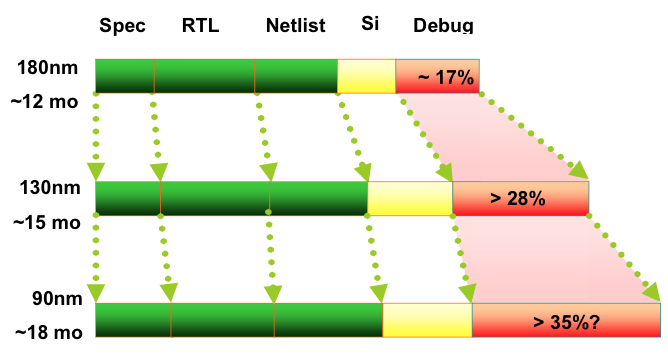
\includegraphics[width=0.7\textwidth]{debugtime.png}
\caption{Silicon Debug vs. time-to-market}
\label{debugt}
\end{figure}

Despite the importance of post-silicon validation, there are not
enough research done to improve its sufficiency.
Post-silicon debugging is difficult because
the amount of internal states engineers can
observe is limited. Several chip-debugging techniques are proposed,
like probe needles and eletron-beam probing.
However, the decreasing silicon sizes and multiple metal layers
in modern silicon structure makes 
debugging techniques based on visual inspection or direct physical contact more difficult\cite{1003792}.
Another commonly used tools are embedded software, mostly done by monitoring
processor bus activity. This method provides only limited observability
of the internal hardware domain\cite{leatherman2003processor}.


A promising alternative is to gather internal signal information
by inserting
 design-for-debug(DfD) into
the circuit design.
Two of the most commonly used techniques are scan chains 
and trace buffers. Detailed definitions and 
debug technologies based on these two techniques will be discussed
in next section.
%However, limited pin-out and
%other architecture factors makes it impossible to have full observability of the system.
%Only a limited number of signals can be observed and traced. This limitation 
%brings challenge in both root cause tracing and debugging process. 

\section{Scan Based Techinique}
The goal of scan based technique is to
reuse the internal scan chains that is
placed in the CUD.
This is original designed to increase
the controllability and observability of the system
during manufacturing test by using the functional pins as scan pins to load 
multiple scan chains concurrently to reduce test time~\cite{nicolici2009design}.


\begin{figure}[h]
\centering
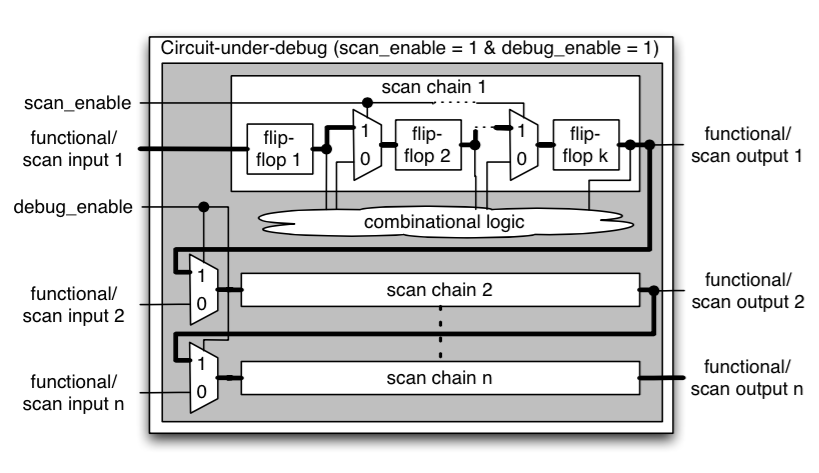
\includegraphics[width=0.9\textwidth]{scanchains.png}
\caption{Scan-based techniques~\cite{nicolici2009design}}
\label{sss}
\end{figure}
For post silicon validation purpose, these
scan chains are concatenated as shown in Figure~\ref{sss},
where internal states will be loaded and unloaded through
a serial interface.
During the post silicon debug process, 
when internal state of the system is needed,
debuggers will stop the system, enable scan chains to capture 
and offload the
internal state elements (scan dump). 
After scan dump is finished, the system should be able
to be resumed from where it was stopped.

During post silicon validation, when the system is deterministic,
allowing test experiment to be able to be stopped and resumed
from any state of interest,
scan chains can be very useful.
However, most of the system failures are not reproducible and 
there is little knowledge about
the cause of failure. Moreover,
system nowadays always contains multiple
clock cycles, stopping the system
without causing any effect on the
system is impractical. For these reasons, scan chains are not
practical for complicate systems.

\section{Trace Based Technique}
Trace buffers is an embedded memory structure that can 
store certain amount of signal data. Once the trace buffer is full, 
the data can be offloaded through low speed device pins for analysis
purpose.

The limitations of scan chains can be address by using embedded logic analyzers (ELA)
using trace buffer. Figure~\ref{tb} shows an example of structures
of ELA.
\begin{figure}[h]
\centering
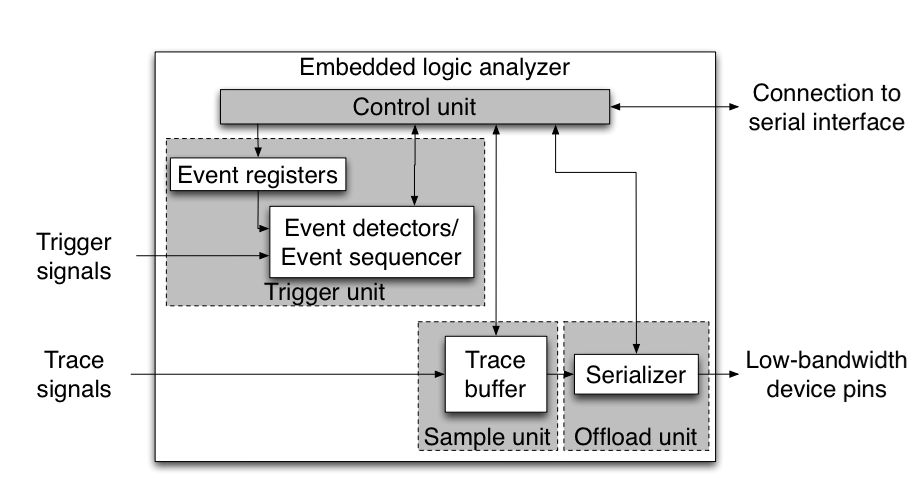
\includegraphics[width=0.9\textwidth]{tracebuffer.png}
\caption{Structure of an embedded logic analyzer~\cite{nicolici2009design}}
\label{tb}
\end{figure}
There are four components inside the ELA: control unit,
trigger unit, sample unit (trace buffer) and offload unit.
Control unit is in charge of all the other unit inside ELA.
Trigger unit monitors a set of trigger signals to detect
trigger event and thus activate the sample unit to
start the data acquisition. The sample unit contains a trace
buffer to record data of selected signals while
offload unit output the data through low-bandwidth device pins.

The amount of data can be acquired by trace buffer is limited by two aspects:
\begin{itemize}
\item
trace buffer $width$: limits numbers of observable trace signals
\item
trace buffer $depth$: limits numbers of samples to be stored.
\end{itemize}
Compared with scan chains, trace buffer allows temporal observability,
making trace analysis possible even when the location of bug
is not known. However, because of the limitation of the trace buffer $width$,
the amount of signals can be observed is limited. This problem can be
mitigated using trace information filtering~\cite{abramovici2006reconfigurable} and compression techniques~\cite{anis2007interactive}.



\section{Related Work}

Our work in this thesis is closely related to communication-centric and
transaction based debug.  An early pioneering work is
described in~\cite{Goossens2007NOCS}, which advocates the
focus on observing activities on the interconnect network
among IP blocks, and mapping these activities to
transactions for better correlation between computations and
communications.  Therefore, the communication transactions,
as a result of software execution, provide an interface
between computation and communication, and facilitate
system-level debug.  This work is extended
in~\cite{Vermeulen2009VLSI-DAT,Goossens2009DATE}.  However,
this line of work is focused on the network-on-chip (NoC)
architecture for interconnect using the run/stop debug
control method.

A similar transaction-based debug approach is presented
in~\cite{Gharehbaghi2012ISQED}.  Furthermore, it proposes an
automated extraction of state machines at transaction level
from high level design models.  From an observed failure
trace, it performs backtracking on this transaction level
state machine to derive a set of transaction traces that
lead to the observed failure state.  In the subsequent step,
bounded model checking with the constraints on the internal
variables is used to refine the set of transaction traces to
remove the infeasible traces.  This approach requires user
inputs to identify impossible transaction sequences, and may
not find the states causing the failure if the transaction
traces leading to the observed failure state is long.
Backtracking from the observed failure state requires
pre-image computation, which can be computationally
expensive.  A transaction-based online debug approach is
proposed in~\cite{Dehbash2014} to address these issues.
This approach utilizes a transaction debug pattern
specification language~\cite{Gharehbaghi2009ICCD} to define
properties that transactions should meet.  These transaction
properties are checked at runtime by programming debug units
in the on-chip debug infrastructure, and the system can be
stopped shortly after a violation is detected for any one of
those properties.  In this sense, it can be viewed as the
hardware assertion approaches in~\cite{Boule2007ISQED}
elevated to the transaction level.

In~\cite{Singerman2011DAC}, a coherent workflow is described
where the result from the pre-silicon validation stage can
be carried over to the post-silicon stage to improve
efficiency and productivity of post-silicon debug.  This
workflow is centered on a repository of system events and
simple transactions defined by architects and IP designers.
It spans across a wide spectrum of the post-silicon
validation including DFx instrumentation, test generation,
coverage, and debug.  The DFx instruments are automatically
inserted into the design RTL code driven by the defined
transactions.  This instrumentation is optimized for making
a large set of events and transactions observable.  Test
generation is also optimized to generate only the necessary
but sufficient tests to allow all defined transactions to be
exercised.  Moreover, coverage for post-silicon validation
is now defined at the abstract level of events and
transactions rather than the raw signals, and thus can be
evaluated more efficiently.  In~\cite{Abarbanel2014DAC}, a
model at an even higher-level of abstraction, {\em flows},
is proposed.  Flows are used to specify more sophisticated
cross-IP transactions such as power management, security,
etc, and to facilitate reuse of the efforts of the
architectural analysis to check HW/SW implementations.




\section{Motivation}

Post-silicon validation is a critical
component of the design validation life-cycle for modern
microprocessors and SoC designs.  Unfortunately, it is also
a highly complex component, performed under aggressive
schedules and accounting for more than $35\%$ of the overall
design validation cost.  Consequently, it
is crucial to develop techniques for streamlining and
automating post-silicon validation activities.

%%explainging why trasfering to system level  transaction
A key component of post-silicon validation of SoC designs is
to correlate traces from silicon execution with the intended
system-level transactions.  An SoC design is typically
composed of a large number of pre-designed hardware or
software blocks (often referred to as ``intellectual
properties'' or ``IPs'') that coordinate through complex
protocols to implement the system-level behavior.  Any
execution trace of the system involves a large number of
interleaved instances of these protocols.  For example,
consider a smartphone executing a usage scenario where the
end-user browses the Web while listening to music and
sending and receiving occasional text messages. Typical
post-silicon validation use-cases involve exercising such
scenarios. 

 An execution trace would involve activities from
the CPU, audio controller, display controller, wireless
radio antenna, etc., reflecting the interleaved execution of
several communication protocols.  On the other hand, due to
observability limitations, only a small number of
participating signals can be actually traced during silicon
execution.  Furthermore, due to electrical perturbations,
silicon data can be noisy, lossy, and ambiguous.
Consequently, it is non-trivial to identify all
participating protocols and pinpoint the interleaving that
results in an observed trace.

%%explainging why should be communication centric verification
With the increasing complexity of modern SoC designs nowadays, 
debugging protocols inside IP
blocks by themselves is not enough anymore. The complexity
of the SOC increasingly resides in the interactions between
the IP blocks. 
Therefore, debug must be conducted
at a higher system level, where the computation threads
and communication threads interact.
 Because the interconnect
implements the communication, and hence the synchronization
between the IP blocks is the natural focus for system-level
debug~\cite{Goossens2007NOCS}.

\section{Contributions}
In this thesis, we consider the problem of reconstructing
protocol-level behavior from silicon traces in SoC designs.
Given a collection of system-level communication protocols
and a trace of (partially observed) hardware signals, our
approach infers, with a certain measure of confidence, the
protocol instances (and their interleavings) being exercised
by the trace.  
The approach is based on a formalization of
system-level transactions via labeled Petri-Nets, which are
capable of describing sequencing, concurrency, and choices
over system events.  We develop algorithms to infer
system-level transactions from traces with missing, noisy,
and ambiguous signal values.

The proposed approach can give silicon debugger
an overview of the system behaviors.
This information can be used to decide
if the system performs the desired behavior and thus
decide the correctness of the design.
Another advantage this approach can provide 
is when traces can not be mapped to 
specifications, indicating that
the specifications are 
not correctly implemented.
When that happens, our proposed
method can provide interesting information
to help root cause the problem.


For the following part of this thesis, 
we present background information on the area of post-silicon validation in Chapter 2. 
Then in Chapter 3 an overview of current flow verification is presented. 
After that, our proposed method and detailed algorithm are explained in Chapter 3 and Chapter 4. 
To demonstrate the correctness of importance of this method, two case studies are constructed and explained
in Chapter 5.
Chapter 6 summarizes our work and talk about our future works. All the flow specifications and protocols used in implementation process will be explained in Appendix.


\chapter{Background}
 \section{Representations of SoC Protocols }
  
 In software engineering field, there are two approaches for representing the system protocols: informal
 and formal representations.
  Informal representation is human friendly and uses common 
  graphical notation for better understandability and easier communication with the client. 
The formal representation, on the other hand, is designed to be machine friendly.
It is usually built on strong mathematical notations and proofs for
more automated verification purpose.

System development usually need to create protocol
in both formal and informal formats. 
At the beginning of the product development cycle, 
system designers create the specification
in graphical (informal) form,
providing good understandability while still
in a standard graphical manner.
After the design is finalized, specifications in formal format is developed
for verification purpose.
Usually it requires manual translation of an informal description to a formal description, 
which 
consumes large amount of time and effort
as modern system involves massive amount of complicate specifications. 
 ~\cite{lsctocpn} introduces a tool that translate live sequence chart
into colored petri-nets that can be used to
speed up the translation process.

 An SoC design involves integration of numbers of IPs that
communicate through complex protocols.  Such system-level
protocols are typically specified in architecture documents
as message flow diagrams. In this thesis, we use the words
``protocol'' and ``flow'' interchangeably.

\begin{figure}[h]
\centering
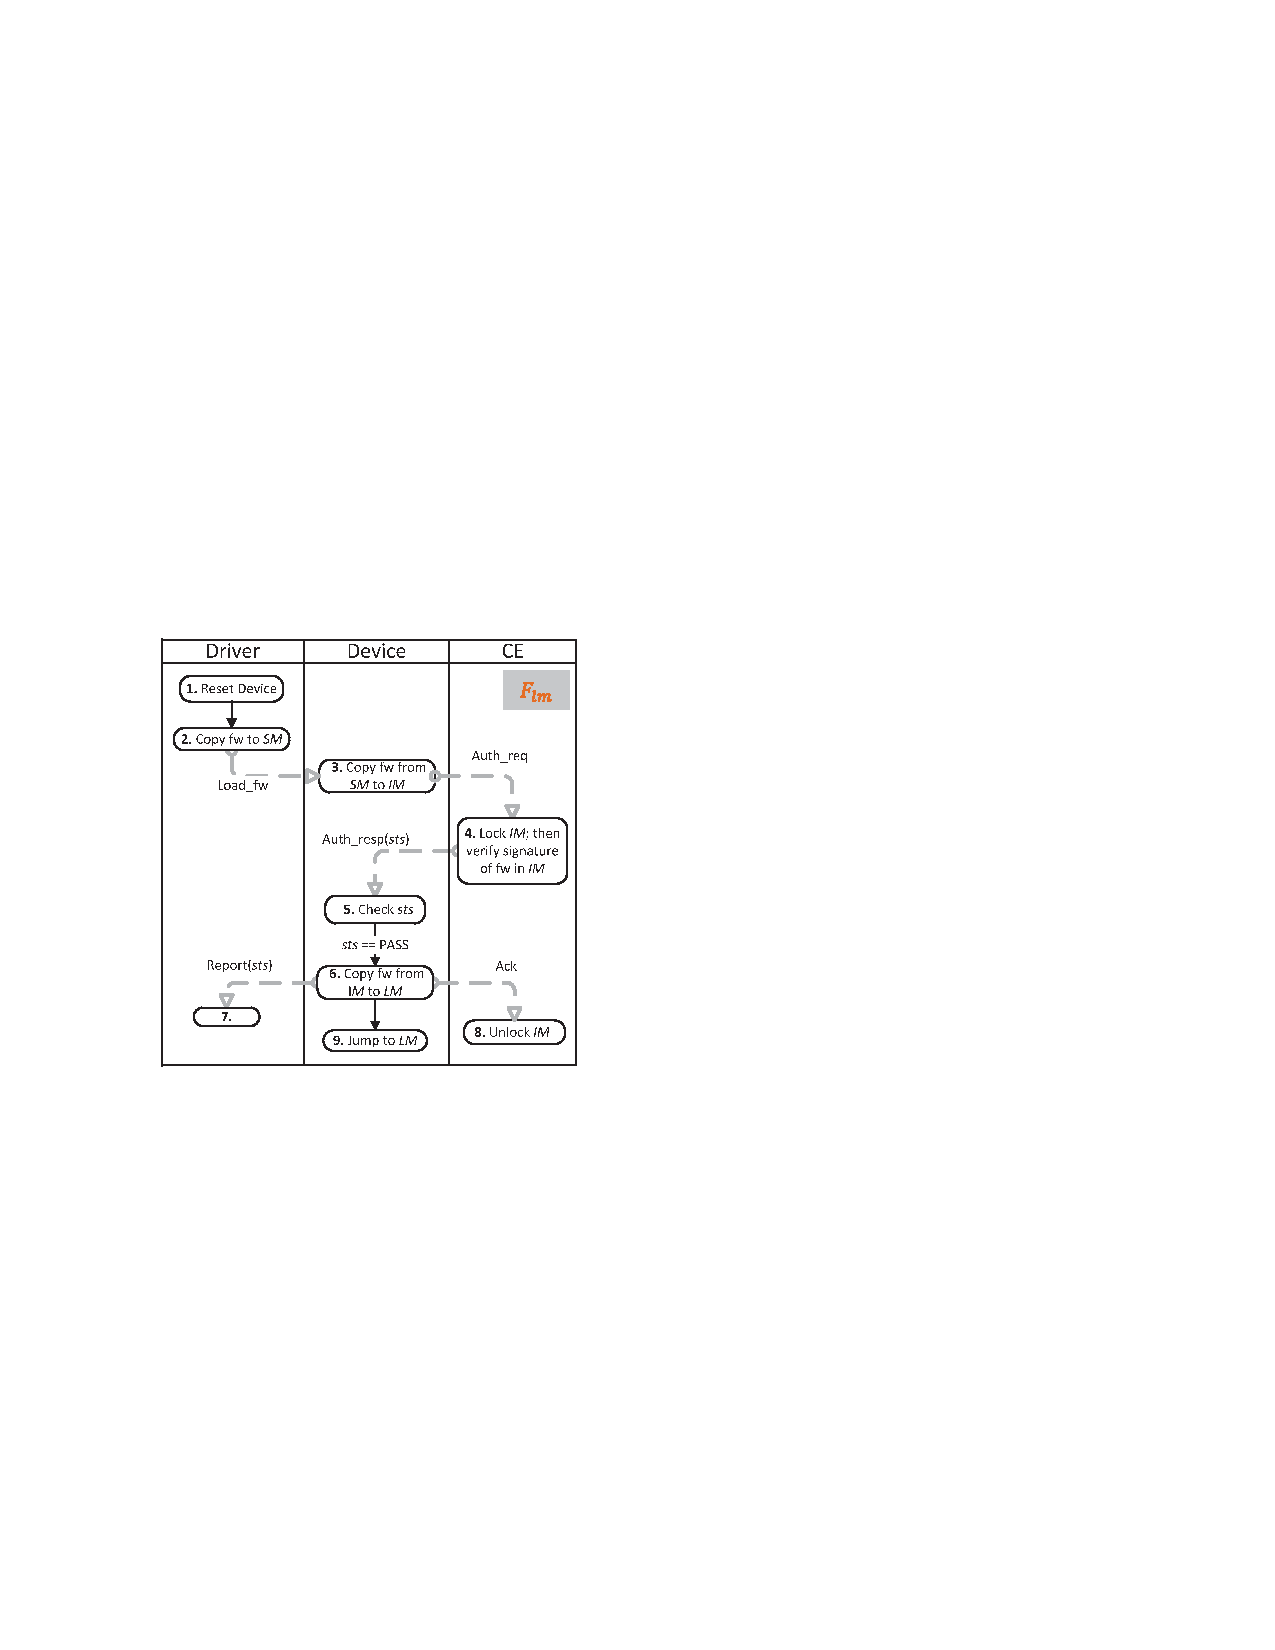
\includegraphics[width=0.5\textwidth]{figures/bpmn-flow-ex}
\caption{A graphical representation of a SoC firmware load protocol~\cite{Krstic14HOST}.}
\label{flowa}
\end{figure}

Figure~\ref{flowa} shows a protocol example that
authenticates and loads a firmware during system boot for
firmware upgrade in Business Process Model and Notation (BPMN). 
BPMN is a standard for business process modeling that provides a graphical notation for
 specifying business processes in a Business Process Diagram (BPD),
 based on a flowcharting technique very similar to activity diagrams from Unified Modeling Language (UML)~\cite{white2004process}.
 
To start this protocol, the Driver resets Device and copies the needed
firmware to a place in System Memory (SM) and notice the Device to load it. With the location of firmware
provided from Driver, Device can retrieve firmware to Isolated Memory (IM) and sends the message $Auth\_req $
to Crypto-engine (CE), providing the location of the copied firmware, and asking for authentication. After verifying 
signature of firmware in IM, CE replys with 
PASS/FAIL status ($sts$). 
Upon receiving the PASS $sts$ such that $sts=PASS$, the Device sends report message to Driver and acknowledgement message
to CE and then jump to the firmware from Local Memory (LM).

The BPMN format used here is a very detailed format, and it is mostly
used in business field. 
A more commonly used graphical format in computer
engineering filed is sequence diagrams.
It represents the
 life cycle of an processor and the interactions between them.
%% Life cycle of an object is represented by a vertical line
 %% and the interaction between objects is represented by 
 %% a horizontal line with an arrow pointing towards the receiver object.
Commonly used sequence diagram include UML sequence diagrams, message sequence 
diagrams and live sequence charts~\cite{lsctocpn}.
 
\begin{figure} [h]
\centerline{
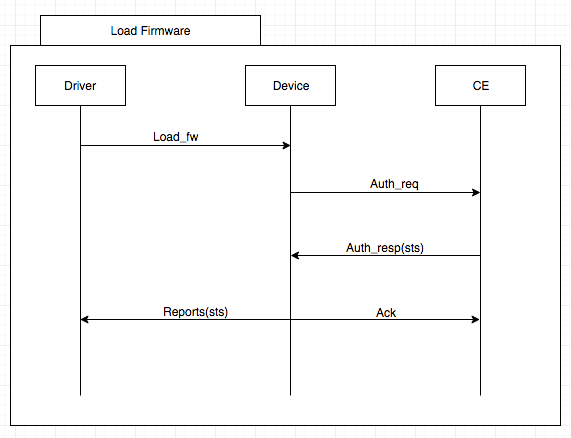
\includegraphics[width=5in]{livesc.png}}
\caption{Protocol in Figure~\ref{flowa} represented in graphical live sequence chart }
\label{livesequence}
\end{figure}
 Figure~\ref{livesequence} shows the live sequence chart representation of the protocol in Figure~\ref{flowa}.
In this graph, we can clearly see the relative time and content of communications between each
components. Unlike the BPMN format in Figure~\ref{flowa}, sequence diagrams is more abstract
as the internal activities of components are not shown.
%%At this time, the initiator sets the $data$ line and then asserts 
%%the $valid$ signal. Once the target samples the $valid$ signal asserted, 
%it is free to sample the value on the $data$ line. 
%After zero or more clock ticks, the target then asserts $ack$ to acknowledge 
%receipt of the data value. At this point, a single clock tick must occur before
 %the $initiator$ can deassert $valid$ and the $target$ can deassert $ack$ since the 
 %data transfer officially occurs on the clock edge on which both $valid$ and $ack$ 
 %are asserted. 
% Again, zero or more clock ticks may occur before the transaction
  %exits by leaving the interface in a state in which $valid$ and $ack$ are both 
  %deasserted. ~\cite{Bunker2005}
  
  
  
\section{Labeled Petri-Nets} \label{petri}
This thesis focuses on algorithmic analysis of system behavior, therefore,
only a formal representation with rigorous
semantics, methods and tools for analysis is needed, such
representation selected by this thesis is the Labeled Petri-Nets (LPN).

A LPN is a formalization of state transition 
system behavior and it is capable of describing sequencing, concurrency, and choices.  
Compared with sequence diagrams,
LPN is more machine friendly, and can be
analyzed using mathematical techniques and tools.

 %--- LPN definition with levels
 
 Formally, an LPN is a tuple $(P, T, s_0, E, L)$  where
 \begin{itemize}
 \item $P$ is a finite set of places,
 \item $T$ is a finite set of transitions,
 \item $s_0 \subseteq P$ is the initial marking.
 \item $E$ is a finite set of events.
 \item $L: T \rightarrow E$ is a labeling function that maps each transition $t \in T$ to an event $e \in E$. 
 \end{itemize}
 
 For each transition $t \in T$, its preset, denoted as $\bullet{t} \subseteq P$, is the set of places connected to $t$, and its postset, denoted as $t\bullet \subseteq P$, is the set of places that $t$ is connected to.  A marking of a LPN is a set of places marked with tokens, and it is also referred to as a state of a LPN. The initial marking $s_0$,
 the set of initially marked places, is 
 also the initial state of the LPN.


 The communication protocol shown
 in~Figure~\ref{flowa} is represented by the LPN
 shown in Figure~\ref{changedb}. 
 This format,
 compared to sequence diagrams,
 is even more abstract. It removes
 all the structure information of a
 system, and represents only communications
activities among the components.
 
 \begin{figure}[h]
\centering
    \includegraphics[width=0.7\textwidth]{try}
  \caption{LPN formalization of protocol in Figure~\ref{flowa}}
  \label{changedb}
\end{figure}

  In this and the
 following figures for LPNs, the labeled circles denote
 places, and the labeled boxes denote transitions.  Each
 transition is labeled with its name and the associated
 event.  Each event has a form of $\langle {\tt src, dest,
   cmd,addr} \rangle$ where ${\tt cmd}$ is a command sent from a
 source component ${\tt src}$ to a destination component
 ${\tt dest}$, and ${\tt addr}$ is the address related to the command
, this can be served as an unique id of the request in some situation.
 The protocol presented in Figure~\ref{changedb} used the
 format of  $\langle {\tt src, dest,
   cmd} \rangle$. Here the ${\tt addr}$ is ignored
   as the command does not have
   any address related.
  In the original protocol specification, the places without outgoing edges
 are {\em terminals}, which indicate termination of protocols
 represented by the LPNs.  The initial marking is
 $\mathit{s_0} = \{p_1\}$.  In this LPN model, only the
 communication portion of the protocol specification is
 represented while the computation portion is ignored.


 The operational semantics of a LPN is defined by transition executions.  
 A transition can be executed after it is {\em enabled}.  
 A transition $t \in T$ is enabled in a state $s$ if every place in its preset is included in $s$, i.e. $\bullet{t} \subseteq s$. 
  The set of enabled transactions in state $s_i$ is denoted as $enabled(s_i)$.
 Execution of $t \subseteq enbled(s)$ results in a new state $s'$ such that 
 \[
 s' = (s - \bullet{t}) \cup t\bullet.
 \]
 
 Let $s'=t(s)$ denote the new state $s'$ after $t$ is executed in $s$.
 When $t$ is executed, the labeled $e$ is emitted.
 Therefore, a sequence of transaction execution
 \[ 
 t_0\ t_1\ t_2\ .....t_i\ ...
 \]
 results in a sequence of events
 \[
e_0\ e_1\ e_2\ .....e_i\ ..., \mbox{such that}\ \forall i \ge 0, t_i \in enabled(s_i) \wedge s_{i+1}=t_i(s_i)
 \]
 Therefore, information exchanges among components in a design can be modeled by
 sequences of LPN transition executions.

  %%@COMMENT This example is for LPNs with guards.
 %The above protocol specification can be made more precise by describing how component~2 would respond without using non-determinism.  For example, the system architect may wish to specify that component~2  responds with $\mathit{msg_2}$ to every sequence of two $\mathit{msg_1}$ for five such sequences in a row.  On the sixth such sequence, component~2 responds with $\mathit{msg_3}$.  The LPN modeling such protocol is shown in Figure~\ref{fig-flow-ex-2}.  An alternative without using auxiliary variables in the transition predicates is by unrolling the loops for the specified number of times; however this would result in a larger and more complex LPN.  


 

\chapter{Flow Guided Trace Interpretation}

 In this chapter,
 we describe a trace analysis method where the observed
 signal traces are interpreted at the level of system
 protocol specifications. In general, the trace analysis can offer
 debuggers a structured view of communications among the
 IP blocks during the SUD execution by deriving the types
 and numbers of system flows activated during System Under Debug (SUD)
 executions from the observed signal traces.

We formalize the trace interpretation problem in terms of labeled Petri-Nets,
 and discuss algorithms to address the problem.
  For pedagogical reasons, here we assume full
   observability of all hardware signals involved in the flow events. 
  In the next chapter we extend the approach
   to consider partial observability.





\section{Post-silicon Trace Analysis}
 In a typical validation setting, the SUD is executed in a test environment until it is
 terminated by the test environment or the system crashes
 due to a failure.  During the execution, a trace on a
 small number of observable signals is streamed off the
 chip for debugging.  
The off-chip analysis
includes two broad phases:
\begin{itemize} 
\item trace abstraction that translates signal traces into flow traces
\item trace interpretation that maps flow traces into flow execution scenarios
\end{itemize}
Trace abstraction maps
a signal trace into higher-level architectural constructs,
\eg, messages, operations, etc. A message such as {\tt
  Authorization request} may be implemented in hardware
through a Boolean or temporal combination of specific
hardware signals in the NoC fabric between {\tt Device} and
{\tt CE}, \eg, as a sequence containing a header, a specific
value of a sequence of data words, etc.  We refer to
such architectural constructs as {\em protocol events} or
{\em flow events}.  Note that due to limited observability,
it may not be possible to map events on a given set of (observed)
hardware signals uniquely to a flow event.  Finally,
signal trace may be a result from several instances of the same
protocol executing concurrently, \eg, a firmware
authentication protocol may be invoked when another instance
of the protocol has not completed.



Trace interpretation entails mapping a sequence of flow events created
during trace abstraction to system-level protocols in order
to identify the set of protocol instances (and their
interleavings) responsible for creating the observed
behavior. The trace interpretation takes a finite trace of flow events
 resulting from the trace abstraction and a set of system
 flows in LPNs $\vec{F}$, and generates a set of possible
 system flow execution scenarios, which is defined in next section.
   A flow execution scenario
 indicates that at a certain point of SUD execution, what
 types of flows and the number of instances of a particular
 flow are activated and their corresponding current states.

The observed traces may help to identify problems in the protocols, 
\eg~an interleaving of some protocol executions
may lead to an unexpected message being sent or cause the
system to crash.  More commonly, one finds a bug in the {\em
  implementation} of the protocol, \ie, a trace inconsistent
with any possible interleaving of the protocol executions.
Identifying these problems involves significant human
expertise, and can often take days to weeks of effort.
The trace analysis method and algorithm presented in this chapter intends to
address that hurdle.



\section{Flow Execution Scenarios}
 The set
of system flows in LPN donates ${\vec{F}}$.  
A {\em flow execution scenario} is defined as a
set $\{(F_{i,j}, s_{i,j})\}$ where $F_{i,j}$ is the
$j$th instance of flow $F_i \in {\vec{F}}$, and $s_{i,j}$ is
a state of $F_{i,j}$.  
A flow execution scenario indicates
the set of protocols and the number of instances of a
particular protocol are activated and their corresponding
current states. 
It represents a system state 
during system execution abstracted on system flow specificatioins.
From debugger's point of view, communication
protocols can be related. For example, a firmware loading
protocol
always happens before a firmware execution protocol.
If a firmware execution protocol happens before firmware loading
protocol, that possibly indicates an error in the system
implementing such portocols.
This information
can be used as an assertion during the debug process.
For this purpose, flow execution scenario also
represents the partial order relations
that define the relative orderings 
between initiation and termination of different flow instances.
This relation can provide helpful information for more
efficient debug.


 Since we assume full observability, we view
an {\em observed trace} $\rho = e_1e_2\ldots e_n$ as a
sequence of flow events.  
 Let
 \[ accept(F_{i,j}, s_{i,j}, e)=
  \begin{cases}
    s'_{i,j}       & \quad \text{if } \exists t, t \in enabled(s_{i,j}) \wedge (L(t) =e) \wedge (s'_{i,j}=t(s_{i,j}))\\
    \emptyset  & \quad \text{otherwise}\\
  \end{cases}
\]
be a function to decide if event $e$ can
be admitted by flow instance $F_{i,j}$ in state $s_{i,j}$.
The function returns the corresponding new state
if event $e$ can be admitted, elsewise
it returns $\emptyset$.
This function is used in the trace analysis algorithm later
in this chapter.

Given an observed trace $\rho$, the
goal of trace interpretation is to construct a set of
candidate flow execution scenarios whose execution can
create the sequence of events in $\rho$.  
In other words, $\rho$ is the result of executing 
the flow instances in those execution scenarios by following 
the corresponding LPN operational semantics
starting from their initial states.

 If every event in $\rho$ is successfully mapped to some
 flow instance, we can say that $\rho$ is $compliant$ with
 the given protocol specifications. When this
 happens, the algorithm returns a set of flow
 execution scenarios.
   On the other hand, inconsistent events may
 also be encountered.  An event $e_h$ is \emph{inconsistent} if
 for each flow execution scenario $\mathit{scen}$,
  the following two conditions hold.
 \begin{enumerate}
 \item For each $(F_{i,j}, s_{i,j}) \in \mathit{scen}$,
   $\mathit{accept}(F_{i,j}, s_{i,j}, e_h) = \emptyset$, and
 \item For each $F_i \in \vec{F}$, $\mathit{accept}(F_{i},
   \mathit{init}_{i}, e_h) = \emptyset$.
 \end{enumerate}

 The inconsistent event $e_h$ is the one produced by SUD execution
 but cannot be mapped to any flow instances no matter how the
 trace prior to event $e_h$ is interpreted. Inconsistent
 events may indicates possible causes of observed system failures.
 When the analysis algorithm finds an inconsistent message,
 it returns the the set of partialy derived execution scenarios along with
 the discovered inconsistent event
 $e_h$.


\section{Flow Guided Trace Interpretation Algorithm}
Given an observed flow trace $\rho$ and the set $\vec{F}$ of system protocol specifications,
Algorithm.~\ref{algo:compliance} describes a basic procedure for
computing a set of compliant flow execution scenarios. 
The algorithm operates by keeping track (in variable
$\mathit{Scen}$) of a set of candidate flow execution scenarios
compliant with each prefix of $\rho$.  At each iteration,
for each event $e_h$ in the observed trace, the algorithm
updates $Scen$ by either updating the state of a member of
$\mathit{scen}$ or by initiating a new flow instance for 
each $scen \in Scen$ with respect to $e_h$ in every possible way.
If $e_h$ cannot be accepted by any existing or new flow instances in $Scen$,
this indicates that trace $\rho$ is inconsistent withe $Scen$.
If event $e_h$ is inconsistent with all existing execution scenarios,
then the algorithm reports that the trace is {\tt  inconsistent} with $\mathit{Scen}$.
 
 Given a trace of flow events $\rho = e_1e_2\ldots e_n$, the
 trace interpretation algorithm starts with an empty set of
 of flow execution scenario $\mathit{Scen} = \emptyset$.
 Then, for each $e_h$ where $1 \leq h \leq n$ starting $h=1$,
 and for each $\mathit{scen} \in \mathit{Scen}$, the
 following two steps are performed.
  \begin{description}
 \item[Step 1]~~For each $(F_{i,j}, s_{i,j}) \in
   \mathit{scen}$, if $\mathit{accept}(F_{i,j}, s_{i,j}, e_h)
   =  s'_{i,j}$, create a new scenario
   $\mathit{scen}' = (\mathit{scen} - (F_{i,j}, s_{i,j}))
   \cup \{(F_{i,j}, s'_{i,j})\}$, which is added into
   $\mathit{Scen}'$.

 \item[Step 2]~~For each $F_i \in \vec{F}$, create a new
   instance $F_{i, j+1}$.  If $\mathit{accept}(F_{i,j+1},
   \mathit{init}_{i,j+1}, e_h) = s'_{i,j+1}$,
   create a new scenario $\mathit{scen}' = \mathit{scen} \cup
   \{(F_{i,j+1}, s'_{i,j+1})\}$, which is added into
   $\mathit{Scen}'$.
 \end{description}
\begin{algorithm}[h]
\setstretch{1.3}
\DontPrintSemicolon
Create an empty scenario $scen$\;
$\mathit{Scen} = \{scen\}$\;
\ForEach {$h, \; 1 \leq h \leq n $} {
	$\mathit{found} \gets {\tt true}$ \;
	$Scen' = \emptyset$\;
	\ForEach {$scen \in Scen$} {
  		\ForEach {$(F_{i,j}, s_{i,j}) \in \mathit{scen}$} {
		$ s'_{i,j} \gets \mathit{accept}(F_{i,j}, s_{i,j}, e_h) $\;
    		\If {$s'_{i,j}\neq \emptyset $} {
				Let $scen'$ be a copy of $scen$\;
      		$\mathit{scen'} \gets \mathit{scen'} - (F_{i,j}, s_{i,j})) \cup (F_{i,j}, s'_{i,j})$\;
      		$\mathit{Scen'} \gets \mathit{scen'} \cup \mathit{Scen'}$\;
      		$\mathit{found} \gets {\tt false}$ \;
    		}
  		}
  		\ForEach {$F_i \in \vec{F}$} {
      	create a new instance $F_{i, j+1}$ \;
	$s'_{i,j+1}\gets\mathit{accept}(F_{i,j+1},\mathit{init}_{i,j+1}, e_h) $\;
      	\If {$s'_{i,j+1}\neq \emptyset  $} {
    			Let $scen'$ be a copy of $scen$\;
				$\mathit{scen'} \gets \mathit{scen'} \cup (F_{i,j+1}, s'_{i,j+1})$ \;
				$\mathit{Scen'} \gets \mathit{scen'} \cup \mathit{Scen'}$\;
        		$\mathit{found} \gets {\tt false}$ \;
      	}
    	}
	}
  \If {$\mathit{found} == {\tt true}$} {
    \Return $\{Scen, e_h\}$\;
  }
  $Scen = Scen'$\;
}
\Return $\mathit{\{Scen, \epsilon\}}$ \;
\caption{$\textsc{Check-Compliance}(\vec{F}, \, \rho)$}
\label{algo:compliance}
\end{algorithm}
\clearpage
After $e_h$ is processed, $Scen = Scen'$, and the above two
 steps repeat for the next event $e_{h+1}$.


 Based on the above discussion, the trace interpretation
 algorithm generates two possible results:
 \begin{itemize}
 \item $\{Scen,\epsilon\}$\ when $\rho$ is compliant with the flow specification $\vec{F}$
 where
 $Scen$  is a set of
 flow execution scenarios, each of which is derived from the observed trace,
 and $\epsilon$ is an empty event indicating non-existence of inconsistent events.
 \item  $\{Scen, e_h\}$\ when inconsistent event occurs
 where
 $Scen$ is a set of partially derived scenarios and
 $e_h$ is the corresponding inconsistent event.
 This result provides valuable
 information for debuggers to root cause system failures.
 \end{itemize}
 
 

\section{Illustration}
To illustrate the basic idea of the trace analysis algorithm,
consider the system flow shown in 
Figure~\ref{changedb}. Let $F_1$ denote such flow.
Suppose that the following flow trace is abstracted from an
observed flow trace.
\begin{equation}
\label{eq:1}
	t_1\;t_2\;t_1\;t_2\;t_3\;t_3\;t_4\;t_5\;t_5\;t_4\ldots
\end{equation} 
This trace is interpreted from the first event to the last in order to derive all possible flow execution
 scenarios.
Here transition names in the LPN are used to represent the 
flow events in the trace.  
At the beginning, event $t_1$ is processed first. 
According to the flow specification $F_1$, 
we know that one instance of such flow $F_1$, $F_{1,1}$, is activated by the SUD 
as $\mathit{accept}(F_{1,1}, init_1, t_1) = p_2$ where $\{p_1\}$ is the initial state of $F_1$. 
The flow execution scenario after interpreting the first event $\mathit{t_1}$ is $\{(F_{1,1}, \{p_2\})\}$.  

Next, the second $t_2$ is interpreted. This event is accepted by
$F_{1,1}$ as $\mathit{accept}(F_{1,1}, {p_2}, t_2) = p_3$.
Next event $t_1$ activates another instance of flow $F_1$, $F_{1,2}$. 
And event $t_2$
 after that can be accepted by $F_{1,2}$, resulting in
the following flow execution scenario:
\[
	\{(F_{1,1}, \{p_3\}),~(F_{1,2}, \{p_3\})\}.
\]
For the fifth event $t_3$, it can be accepted by both $F_{1,1}$ 
and $F_{1,2}$. Therefore,
two execution scenarios can be derived as showed below.
\[
\begin{array}{l}
	\{(F_{1,1}, \{p_4, p_5\}),~(F_{1,2}, \{p_3\})\} \\
	\{(F_{1,1}, \{p_3\}),~(F_{1,2}, \{p_4, p_5\})\}.
\end{array}
\]
After handing the following event $t_3$, the above two execution scenarios
are reduced to the one as shown below.
\[
	\{(F_{1,1}, \{p_4, p_5\}),~(F_{1,2}, \{p_4, p_5\})\}.
\]
After processing the next event $t_4$, the two execution scenarios below
can be derived:
\[
\begin{array}{l}
	\{(F_{1,1}, \{p_6, p_5\}),~(F_{1,2}, \{p_4, p_5\})\} \\
	\{(F_{1,1}, \{p_4, p_5\}),~(F_{1,2}, \{p_6, p_5\})\}.
\end{array}
\]
Next, processing the following event$t_5$ leads to execution scenarios derived 
from those shown above :
\[
\begin{array}{l}
	\{(F_{1,1}, \{p_6, p_7\}),~(F_{1,2}, \{p_4, p_5\})\} \\
	\{(F_{1,1}, \{p_4, p_7\}),~(F_{1,2}, \{p_6, p_5\})\}\\
	\{(F_{1,1}, \{p_6, p_5\}),~(F_{1,2}, \{p_4, p_7\})\} \\
	\{(F_{1,1}, \{p_4, p_5\}),~(F_{1,2}, \{p_6, p_7\})\}.
\end{array}
\]
Similarly, next event $t_5$ reduces the execution scenarios above to the following ones:
\begin{equation}
 \label{eq:2}
 \begin{split}
	\{(F_{1,1}, \{p_6, p_7\}),~(F_{1,2}, \{p_4, p_7\})\} \\
	\{(F_{1,1}, \{p_4, p_7\}),~(F_{1,2}, \{p_6, p_7\})\}.
\end{split}
\end{equation} 
Eventually, after handling the last event $t_4$ the execution scenario below is
derived.
\[
	\{(F_{1,1}, \{p_6, p_7\}),~(F_{1,2}, \{p_6, p_7\})\}
\]

In this example all flow events are successful mapped and every flow scenario reached its
end state. The result shows that
two instances of the firmware loading flow
are activated during the system run
and finished correctly. While no error happens
during the analysis process, debuggers
can use this
result to check if the numbers of flow instances are
correct compared to the expected data
extracted from verified simulation.
This process involves checking types of
protocol specification activated and
numbers of flow instances of each protocol.
Moreover, depends on the correlation between
protocols, together with recorded order of each flow instance's
start and finish time, debugger can judge if
the system functions correctly. 

Now suppose that system generate a trace same as the previous one in (~\ref{eq:1} )
except that the last event is $t_3$ instead of $t_4$. The new traced is showed below:
\[
	t_1\;t_2\;t_1\;t_2\;t_3\;t_3\;t_4\;t_5\;t_5\;t_3\ldots
\]  
The same execution scenario as in (\ref{eq:2}) are derived after the first nine elements are handled:
\[
\begin{array}{l}
	\{(F_{1,1}, \{p_6, p_7\}),~(F_{1,2}, \{p_4, p_7\})\} \\
	\{(F_{1,1}, \{p_4, p_7\}),~(F_{1,2}, \{p_6, p_7\})\}.
\end{array}
\]
 However, neither of these two existing scenarios can accept
 $t_3$. Furthermore, because no new flow instances can
 be created such that $t_3$ can be accepted in the initial
 states. Therefore $t_3$ is regarded as an inconsistent event.
 
When an inconsistent event happens, debuggers can make use
of the current partially derived scenarios and the inconsistent flow event to
guess possible causes and the potential problematic 
components in the system.
Based on this information, debuggers can 
select a new set of observable signals in order to better visualize the activities around
the suspicious components in a new SUD execution.
The new observed traces can help
debuggers better understand the problem,
and may eventually lead to locating the
root cause of the problem.
  
\chapter{Trace Analysis Under Partial Observability}

In hardware that implements a given system flow
 specification, a flow event is assumed to be implemented as an event or a
 sequence of events on a set of hardware signals.  
 However, in post-silicon debug, 
 it is impossible to observe all or a
 large number of
 signals. 
 
 
 %This limited observability is due to:
 %\begin{itemize}
% \item Limitation of the interface: there are limited number of pins on the boundary of chip available for observation.
% \item Speed frequency difference: the big speed frequency gap between chip and interface may lead to data lost. 
% \end{itemize}

 
 In this chapter, the analysis algorithm is extended by adapting
 trace analysis method presented in the previous chapter to deal
 with signal traces of partial observability. 
Hereafter, the term {\em flow traces} is used to refer to
traces of flow events, and {\em signal traces} refers to traces of signal events
observed from system execution.

\section{Mapping Individual Signal Events to Flow Events}

A signal event is defined as a state on or an
assignment to a set of signals.
In general, a signal trace of partial observability is a sequence of signal events
such that the values of non-observable signals are unknown. In this case, all possible values of those signals
are considered for every signal event during trace analysis. 
Thus we can say that one partially observed signal
 trace can be mapped to a set of fully observable signal traces.

Consider the following example for
mapping individual signal events to flow events.
Suppose that there are three flow events:
$e_1$, $e_2$, and $e_3$, which are implemented in hardware
by the signal events shown in the list below.  We use
Boolean expressions to represent signal events for the
discussion.
\[
\begin{array}{cl}
e_1: & abc\\
e_2: & \bar{a}bc\\
e_3: & a\bar{b}c
\end{array}
\] 
Suppose that only signals $b$ and $c$ are observable, and we
obtain the following trace
\[
\rho = bc\ bc \ \bar{b}c
\]
Since $a$ is not observable, both possible assignments to $a$
need to be considered
when these signal events are mapped to 
flow events.

The first and second signal events $bc$, can be
mapped to possible signal events with both values of $a$ assigned:
$abc$, $\bar{a}bc$.
The first signal event $abc$ can be mapped to $e_1$.
While $\bar{a}bc$ can be mapped to $e_2$. Therefore,
signal event $bc$ with $a$'s value unknown can be mapped to
 $\{e_1,e_2\}$. 

Similarly, the third signal event $\bar{b}c$ can be mapped to 
$a\bar{b}c$
and
$\bar{a}\bar{b}c$,
respectively.
In this case $a\bar{b}c$ is mapped to $e_3$. On the other hand,
$\bar{a}\bar{b}c$ can not be mapped
to any flow event, therefore,
this interpretation of signal $a$ is invalid, and is ignored.

Based on the above discussion,,
this signal trace $\rho$ is abstracted to four possible flow traces: $\{e_1,
e_2\} \times \{e_1, e_2\} \times \{e_3\}$.
%Hereafter, we will not repeat the process of mapping partial observed signal event to set of 
%fully observed signal events. 


\section{Mapping Sequences of Signal Events to Flow Events}
Next, we consider the case where a flow event is implemented by
a sequence of signal events
when the flow event models a transaction that
takes a number of signal events to accomplish. For example,
a flow event that represents a message sent from component
$A$ to component $B$ with handshake protocol consists
of two steps: (1) component $A$ sets the valid bit to 1 together with
the command,
(2) and component $B$ sets the acknowledgement
signal to 1.

Now suppose that two
flow events are implemented by two sequences of signal events as
defined in the list below.
\[
\begin{array}{cl}
e_4: & abc\ \bar{a}bc\\
e_5: & abc\ abc\ abc\ \bar{a}bc\\
\end{array}
\] 

Again, assume that $a$ is not observable, and suppose that an observed trace
on signals $b$ and $c$ is obtained as shown in (\ref{eq:8}).

\begin{equation}
\label{eq:8}
\rho=bc\ bc\ bc \ bc
\end{equation}



The mapping function takes the signal trace $\rho$, index of next signal event $i$
and mapping table of flow events and signal events as
input, and returns a set of pairs ($e,i'$) where
$e$ is a flow event mapped from possible sequence of signal events
starting from signal event at index $i$ and $i'$ is
the index of next signal event to be considered.
Starting from the current signal event with index $i$, consider all prefixes of
increasing length up to Max, map each $pref(\rho,k)$ to
a flow event.
If successful, return $(e,i')$ such that $i'=i+k$.
Here $Max$ is the length of the longest sequence of signal events that implement a flow event.


In this example, assume the index for the first signal event is 0. 
The given mapping relationship between the flow events and the signal events shows
the length of a signal event for a flow event is either two or four. Therefore in this case
value of $Max$'s is 4.
The function takes $\rho, Mapping\ table$ and $i$ with value set to 0 as input.

Start with the first signal event $pref(\rho,1)=bc$, it can not be matched to any
flow event. 
Next round, the new sequence $pref(\rho,2)=bc\ bc$ is considered,
by looking up the mapping table,
this can be mapped to $e_4$, and $i'=i+2$ is 2.
After that, sequence $pref(\rho,3)=bc\ bc\ bc$ can not be mapped to any flow event.
Last, as the length of new sequence $bc\ bc\ bc\ bc$'
reaches $Max$ 4. This new sequence can be mapped to $e_5$, and the
index $i'$ of the next signal event to consider is $i+4=4$.
Subsequently, the function terminates and
returns the set of pairs:
\[
\{(e_4,2),(e_5,4)\}
\]

The pair $(e_5,4)$ reaches the end of the signal traces,
therefore the mapping ends.
For $(e_4,2)$, the mapping function is applied to $\rho$
with index $i$ changed to 2 and
it
returns $\{(e_4,4)\}$.
After combining the previous result, two flow traces
are derived from $\rho$ as shown below.
\[
\{e_4\ e_4, \ e_5\}
\]

%
%\section{Mapping Sequence of Gapped Signal Events to Flow Events}
%
%Most of the time, the speed of data generation is much faster
%than speed of pins outputting data. 
%Therefore, when the speed of data being generated
%is much faster than it is transported via the
%output pin, there will be a certain period of
%time where data can not be transported, therefore lost while the
%debug interface is busy outputting the previously generated data.
%This will result in a gap in the signal trace.
%
%To discuss about how
%the analysis algorithm do for situation like this,
%we will use flow events $e_4$ and $e_5$ from previous section as an example.
%\[
%\begin{array}{cl}
%e_4: & abc\ \bar{a}bc\\
%e_5: & abc\ abc\ abc\ \bar{a}bc\\
%\end{array}
%\] 
% 
%Given an observed trace with signal $a$ not observable as it is shown below
%\[
%\begin{array}{cl}
%bc\ \textvisiblespace\  \textvisiblespace\ bc\ bc\
%\end{array}
%\]
%
%The $\textvisiblespace$s in the signal trace indicate the gap with maximum two signal events.
%The maximum number of possible signal events happened in the gap is assumed to be
%provided by the debugger's insights of the system.
%For this situation, the analysis algorithm will iterate through each $\textvisiblespace$, considering all possible 
%signal
%events and try to map it to flow events. 
%This process will stop when the signal events
%can be mapped to a flow event, and
%the newly mapped flow event can be 
%mapped to an existing scenario or start a new scenario. 
%If no mapped flow event can be
%accepted from the scenario
%after considering the last $\textvisiblespace$, then we conclude there is an error.
%
%For this example, there are four possibilities: $bc\ b\bar{c}\ \bar{b}c\ \bar{b}\bar{c}$ 
%for each of the $\textvisiblespace$.
%Only $bc$ can be accepted since flow event $e_4\ and\ e_5$ only accept $bc$.
%So start with the first $\textvisiblespace$, the new signal trace are
%\[
%\begin{array}{cl}
%bc\ bc\ bc\ bc\
%\end{array}
%\]
%This is same with the previous section in equation \ref{eq:4}.
%And same result will be generated after mapping the first
%four signal events:
%\[
%\begin{array}{cl}
%flow\ events & next\ index\ of\ signal\ event\\
%e_4\ e_4 & 4\\
%e_5 & 4\\
%\end{array}
%\]
%
%Hereafter the algorithm will try to map above flow events
%to scenarios. If inconsistent flow event happens
%during the mapping process, the algorithm will
%go back to the iteration and start with the second
%$\textvisiblespace$. A new signal trace will be generated:
% \[
%\begin{array}{cl}
%bc\ bc\ bc\ bc\ bc\
%\end{array}
%\]
%After applying the same algorithm from previous section,
%following result will be generated:
%\[
%\begin{array}{cl}
%flow\ events & next\ index\ of\ signal\ event\\
%e_4\ e_4 & 4\\
%e_5 & 4\\
%\end{array}
%\]
%
%The last event $bc$ can not be mapped to any flow event.
%For this situation, the algorithm will halt
%the analyzing process and report the error.
%




\section{Generalized Trace Analysis Algorithm}%

As shown in the previous section,
more
than one flow trace can be derived from
a signal trace under partial observability.
The number of flow traces can
grow exponentially as the system
complexity increases and the number of
signals being able to be observed remains
the same.
Flow traces are usually very long
and thus requires a lot of time
to interpret, the large number
of flow traces can drastically
increase the analysis time.
To address this problem,
our research combines trace abstraction
with trace interpretation and
a new generalized algorithm is
presented next.
 The detailed algorithm pseudocode
is shown in Algorithm~\ref{algo:gene}.

\begin{algorithm}
\setstretch{1.3}
\DontPrintSemicolon
Create an empty scenario $scen$\;
$\mathit{Scens} = \{(scen,0)\}$\;
$Scens\_final=\emptyset$\;
\While{$Scens\neq \emptyset$} {
 	$get\ (Scen,i)\in Scens$\;
	
	$(E,I)\gets Map(\rho,i,Flow\_Map)$ \;
	\ForEach{$(e,i')\in (E,I)$}{
		$Scens'\gets Flow\_Analysis(\vec{F},Scen,e)$\;
		
		
		\If{$Scens' \neq \emptyset$}{
			\eIf{$i' = |\rho|$}{
				$Scens\_final=Scens\_final\cup (Scens',i')$
			}{
			$Scens=Scens\cup (Scens',i')$\;
			}
		}
		
	}
	$Scens= Scens - (Scen,i)$\;
	$Scens\_d=Scens\_d\cup (Scen,i)$\;
 }
\eIf {$Scen\_final = \emptyset$}{
	\Return $(Scens\_d, true)$\;
}
{
\Return $\{Scen\_final, false\}$\;}
\caption{$\textsc{Generalized-Check-Compliance}(\vec{F}, \, \rho)$ }
\label{algo:gene}
\end{algorithm}




\begin{algorithm}[h]
\setstretch{1.3}
\DontPrintSemicolon
$Result= \emptyset$\;
$pref=\epsilon$\;
	\For{$i\to 0 ... min(Max, |\rho|-1)$}{
		$pref=\rho [h,h+i]$\; 
		\ForEach{$(e,\sigma)\in Flow\_Map$}
		{ 		
		\If{$i==|\sigma|$}{
			$flag=true$\;
			\ForEach{$k\in 0... i-1$}{
				\If{$\sigma[k] \nRightarrow pref[k]$}{
					$flag=false$\;
					$break$\;
				}
			}
			
			\If{$flag == true$}{
				$Result=Result\cup (e, h+i)$\;
			}
		}
		
		}
	}
\Return $Result $\;
\caption{$Map(\rho, h, Flow\_Map)$}
\label{map}
\end{algorithm}



\begin{algorithm}[h]
\setstretch{1.3}
\DontPrintSemicolon
$Scen\prime = \emptyset$\;
	\ForEach {$scen \in Scen$} {
  		\ForEach {$(F_{i,j}, s_{i,j}) \in \mathit{scen}$} {
		$s'_{i,j} \gets \mathit{accept}(F_{i,j}, s_{i,j}, e_h) $\;
    		\If {$s'_{i,j}\neq \emptyset $} {
				Let $scen'$ be a copy of $scen$\;
      		$\mathit{scen'} \gets (\mathit{scen'} - (F_{i,j}, s_{i,j})) \cup (F_{i,j}, s'_{i,j})$\;
      		$\mathit{Scen\prime} \gets \mathit{scen'} \cup \mathit{Scen'}$\;
    		}
  		}
  		\ForEach {$F_i \in \vec{F}$} {
      	create a new instance $F_{i, j+1}$ \;
	$s'_{i,j+1}\gets\mathit{accept}(F_{i,j+1},\mathit{init}_{i,j+1}, e_h)$\;
      	\If {$ s'_{i,j+1}\neq \emptyset  $} {
    			Let $scen'$ be a copy of $scen$\;
				$\mathit{scen'} \gets \mathit{scen'} \cup (F_{i,j+1}, s'_{i,j+1})$ \;
				$\mathit{Scen\prime} \gets \mathit{scen'} \cup \mathit{Scen'}$\;
      	}
    	}
	}
\Return $Scen\prime$
	
\caption{$Flow\_Analysis(\vec{F},Scen,e)$}
\label{func}
\end{algorithm}

In this generalized algorithm, multiple instances are used. 
In line number 2, $Scens$ is a set of pairs $(Scen, i)$. Each pair represents scenario $Scen$
extracted for signal trace from beginning to index $i$. The pairs are ordered
by $i$ in ascending order.
In line number 6,
$Flow\_Map$ is the mapping table between flow event and signal events, and is a set
of ${(e,\sigma)}$ where $e$ is the flow event, and $\sigma$ is the correspond sequence of
signal events. In the following sections, $\sigma[i]$ is used
to present $i$th signal event in $\sigma$.
In line number 3,
$Scen\_final$ is created as a set of pairs $(Scen, m)$ represent final scenario after finish processing all signal traces,
together with size of the signal events.
In line number 18,
 $Scens\_d$ is created to hold a set of pairs  $(Scen, i)$ that are deleted from $Scens$

A new $Map(\rho, h, Flow\_Map)$ is created
to find matching flow events from 
signal events start at index $h$.
This function returns a set of pairs of K, each pair in K
consists of $(e, i)$ where $e$
is a matched flow event,
and $i$ is the corresponding positions of next signal event
to be considered. 

Here the mapping algorithm uses the breadth first searching algorithm,
meaning for each signal event, the algorithm considers all
possible flow traces that can be mapped to and calculate the next signal event index.
When all possible flow events are extracted, the algorithm
goes through each of the possible index of signal event and
do the same process again.
Detailed algorithm is shown in Algorithm~\ref{map}.
Symbol $\Rightarrow$ in line number 9 is a function means implying. For example $r_i \Rightarrow s_i$
means a fully observed signal event $r_i$ can imply partially observed signal event $s_i$
In line number 4, $\rho [h,h+i]$ is used as a function that returns a sequence of signal event starting from index h to index h+i in $\rho$

Another function $Flow\_Analysis(\vec{F},Scen,e)$ is
also used. This function takes current scenario set $Scen$, event $e$ and flow specification $\vec{F}$
as input, and returns a new set of scenarios produced after executing event $e$. Details
of the function are shown in Algorithm~\ref{func}.

This algorithm terminates in two conditions:
(1) When all signal events are processed and the algorithm returns
($Scen\_final$,$false$). $Scen\_final$ is the set of final scenarios, and $false$ indicates
no existent of inconsistent event.
(2) When inconsistent event happens, the algorithm returns the set of
deleted scenarios  $Scen\_d$ where inconsistent event happened and
boolean with value $true$ indicates existent of inconsistent event.









\clearpage
\section{Difficulties and Solutions}
It is clear from above that a partial trace is viewed as a
set of flow traces, and Algorithm~\ref{algo:compliance} can
be suitably extended to work with flow traces to obtain the
set of candidate flows.  However, applicability of the
algorithm in practice can be gated because the number of
potential flow execution scenarios generated under partial
observability may be enormous.  Note that this is not a
limitation of the algorithm; if the observability of
critical events is poor there simply {\em are} too many flow
execution scenarios compliant with the observed trace.

Nevertheless, we need to address the issue to make trace
interpretation (whether automatic or not) practicable.
There are two potential approaches: (1)~better selection of
post-silicon trace observability, and (2)~use of system
insights during validation. 
Trace signal selection itself
is an important and orthogonal topic~\cite{nicolici,basu},
and finding an automated way of signal selection algorithm can be one 
of our future research direction. We briefly describes impact of signal selection
and how the debuggers'
insights of a system's architecture can help to address the
complexity issue in the trace interpretation in next two sections.

\section{Trace Signal Selection}
Trace signal selection in this research is done manually by the debugger. 
This is process is labor-intensive and heavily relied on the debugger's insights.
During the experiment conducted by this research,
different sets of signals was selected and tested on the algorithm.
The best sets of signals can be selected
by comparing the numbers of different scenarios returned
after analyzing the signal traces.
This ad-hoc method, even though the debuggers' knowledge
is of great help for debugging process, 
can not guarantee the quality of the selected trace signals.
For bugs that are not expected, it is nearly impossible to select
signals that are related to them during the design phase.
Therefore, we need to have a least some trace signals
that are selected in an automated manner without
debuggers' insights to achieve effective bug detection.
 
Most of the current signal selection algorithm are done in low-level and using 
SSR (State Restoration Ratio)  as 
their metric. 
SRR measures signal selection algorithm by counting
the number of design states able to be reconstructed
 from the signals observed. 
However, as explained in 
 ~\cite{forestMa}, because SSR treats all signal equally and thus always favor big arrays,
 it may not be very helpful to restore useful system states for our case. We need a tool that can 
 restore the maximum states in system level and thus lead to less scenarios.
 
 ~\cite{forestMa} proposed an interesting algorithm based on Google's PaperRank system. 
 This algorithm rank each signal based on their connectivity to other instances and chose 
 those most valuable signals. However, this algorithm does not support system level assertions
 hence may not be able to chose the best signals to restore system level state in our case.
  ~\cite{signalselect} mentioned another way of 
signal selection in system level using linear program formulation. This method focus on communications
 between IPs and try to maximize the coverage of each protocol messages. Combining this method
 on our system and evaluate its performance is one of our future jobs.

\section{Interactive Trace Interpretation}

Post-silicon validation is performed by debuggers with deep
knowledge about the system's architecture and
micro-architecture, and the test environment.  Two key
insights are (1) the maximal number of instances of a flow
activated in the test environment, and (2)~the mutual
relationship between two flows.  For example, the test
environment may not allow multiple instances of firmware
authentication to operate concurrently, or a flow involving
audio and Web browsing to initiate until the flows
participating in boot are completed.  Our framework permits
incorporating such insights as constraints in trace
analysis; flow execution scenarios that violate these
constraints are ignored.  These insights can lead to two
advantages.  First, they help to reduce the potentially
large number of partial scenarios generated during the trace
interpretation step, thus making the analysis more
efficient.  Second, they allow the debugger to quickly
filter out uninteresting combinations of flows and focus on
interesting interleavings.

This approach can be flexible in that it allows a debugger
to analyze the observed traces in a trial-and-error manner
if the precise knowledge of the system (micro-)architecture
is hard to come by.  For instance, the debugger might
initially make a very restricted assumption on how the SUD
executes a flow specification, and these assumptions can
potentially lead to an empty set of flow execution
scenarios.  Depending on which of these assumptions
triggered during the trace interpretation step, the debugger
can study these assumptions more carefully, and relax some
or all of them for the next run of analysis.  This iteration
can be repeated as many times as necessary until some
results deemed meaningful are produced.


 Alternatively, if all derived execution scenarios seem to be
 plausible, the implication that a debugger may draw from
 this result is that the failure may be independent of the
 flows being observed.  Therefore, the testing environment
 can be adjusted in order for a different part or different
 behavior of the SUD to be observed.  This idea, closely
 related to trace signal selection, is critical for
 post-silicon validation, and a detailed discussion can only
 be presented in a separate paper.



\chapter{Case Studies}
This chapter demonstrates the uses of our proposed
algorithm on two different model. In the
first section, the trace analysis algorithm is applied to
a transaction leveled model of a simple SoC
built on the simulator GEM5. 
In the next section, 
a more detailed RTL model is conducted to
further test the effeteness of our algorithm.

\section{A Transaction-Level Model of a Simple SoC in GEM5}
\begin{figure} 
\centerline{
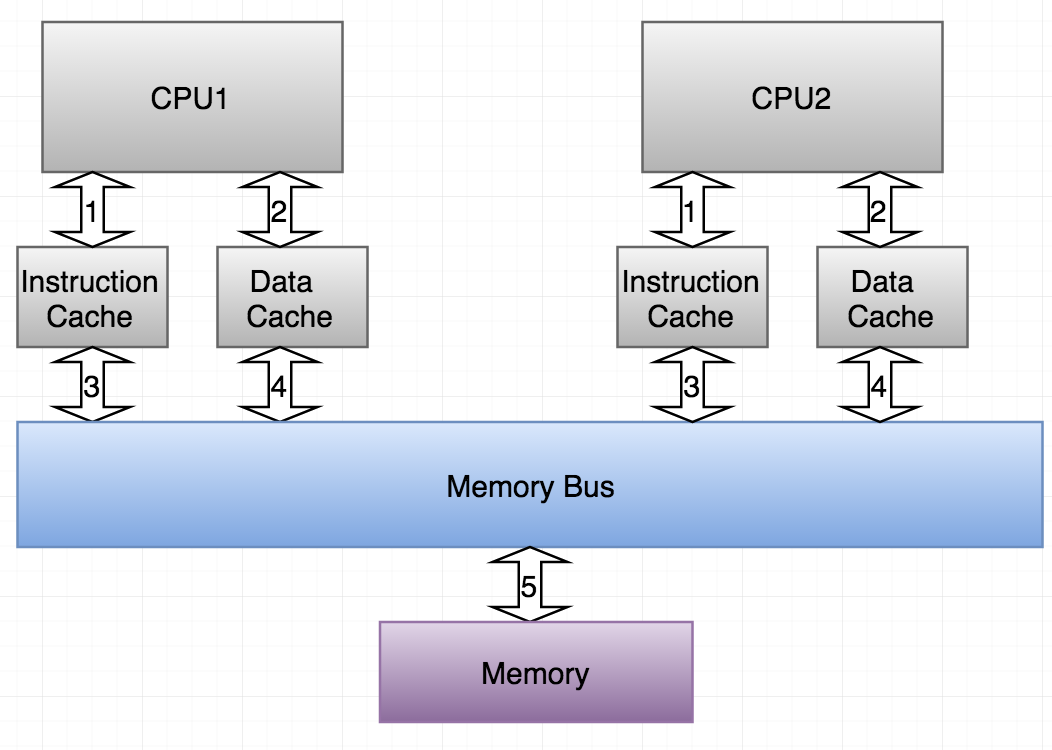
\includegraphics[width=5in]{Gem5.png}}
\caption{Structure of the SoC TLM}
\label{SoC}
\end{figure}

To determine the efficiency of the trace analysis method for
a realistic example, a transaction level model of a SoC is
constructed within the GEM5 environment~\cite{Binkert2011}.
The GEM5 simulator is a modular platform for computer-system architecture research, 
encompassing system-level architecture as well as processor micro-architecture.
This SoC model, as shown in Figure~\ref{SoC}, consists of two
ARM Cortex-A9 cores, each of which contains two separate
16KB data and instruction caches.  The caches are connected
to a 1GB memory through a memory bus model.  Components
communicate with each other by sending and receiving various
request and response messages.  In order to observe and
trace communications occurring inside this model during
execution, monitors are attached to links connecting the
components.  These monitors record the messages flowing
through the links they are attached to, and store them into
output trace files.


In this SoC design, there are nine interfaces in total and each 
interface is attached with a monitor.
 By combining the information from all of the nine communication monitors, 
 the traces of the communication activities between each component
 are obtained.
As a virtualized SoC platform, GEM5 has three types of accesses supported by
its communication interface:
timing, atomic and functional.
Timing accesses is the most detailed one,
it reflects the simulator's best effort for realistic timing
and includes the modeling of queuing delay and resource contention.
Once a timing request is successfully sent,
at some point in the future the device that sent the request will get a response~\cite{gem5}. 
Atomic access is a faster access compared to timing request with no delay.  
This accesses are used for fast forwarding and warming up caches and return an approximate time to complete the request without any resource contention or queuing delay.
When an atomic access is sent,
the response is provided when the function returns~\cite{gem5}.
Functional accesses are used for loading binaries, examining and changing variables in the simulated system,
and allowing a remote debugger to be attached to the simulator.
Those functions are not used for
our simple SoC.
In our experiment, we specified all the communications to be timing access
so the system has 
the most realistic timing.


For this model, we consider the flow specifications
describing the cache coherence protocols supported in
GEM5 that is used to build the model in Figure~\ref{SoC}.
The GEM5 cache coherence protocols can be found at~\cite{gem5}.
These protocols and their corresponding LPN descriptions can also be found
in Appendix A.
These flow specifications describe data/instruction read
operations and data write operations initiated from CPUs.
Three such flows describe the cache coherent protocols for
each CPU.  Since there are two CPUs, there are six flows in
the model.



We wrote one simple concurrent programs with two threads, one for each CPU
to exercise the flows.
The program assigned to CPU1 read one file three times and do some modifications to
the content of the file. 
CPU2's does the same read and write functionalities to the same file, the only difference is that CPU2 modifies the file first and then
perform the reading function. 

After this model is executed with the simple concurrent program, 
the trace analysis is applied to traces with different observabilities
collected from this model.  The runtime results are shown in Table~\ref{table-results}.
The first column shows the results from analyzing the trace with the full
observability, while the next three show the result from 
analyzing traces with different partial observability assumptions.

In the first experiment, full observability is assumed.
After the SoC model finishes executing the program, there
are totally $343581$ messages collected in the trace file.
Not all of the messages are relevant to the flow
specification as many are used by GEM5 to initialize its
simulation environment.  After removing those irrelevant
messages, the number of messages in the trace file is to
reduced to $121138$.

\begin{table}[h]
\begin{center}
\begin{tabular}{|c|c|c|c|c|}
\hline
	&	F-Obs. & \begin{tabular}{c}P-Obs. \\ No Amb.\end{tabular} & \begin{tabular}{c}P-Obs. \\ Amb.~1\end{tabular} & \begin{tabular}{c}P-Obs. \\ Amb.~2\end{tabular} \\
\hline
\hline
Time & $3$ & $2.78$ & $896$ & $<1$\\
\hline
Mem & $12$ & $10$ & $420$ & $9$\\
\hline
	
\end{tabular}
\end{center}
\label{table-results}
\caption{Runtime Results of Trace analysis. Time is in seconds and memory usage is in MB.}

\end{table}%


The time taken to remove the irrelevant messages from the
trace is negligible.  The total runtime and the peak memory
taken by the trace analysis algorithm on the reduced
trace are 3 seconds and 12MB, respectively.  Only one flow execution
scenario is extracted, and 
Table~\ref{table-case-2} shows the number of flow instances contained in that
scenario for the six 
flows describing cache coherent operations initiated from both CPUs.
\begin{table}[tb]
\caption{The number of flow instances derived by the trace analysis with the full observability.}
\begin{center}
\begin{tabular}{|l|c|}
\hline
Flows & $\#$Instances \\
\hline
\hline
CPU1 Data Read			&  $17582$\\
CPU1 Instruction Read		&  $4002$\\
CPU1 Write				&  $3370$\\
\hline
CPU2 Data Read			&  $17386$\\
CPU2 Instruction Read		&  $3955$\\
CPU2 Write				&  $3308$\\
\hline
\end{tabular}
\end{center}
\label{table-case-2}
\end{table}%

In the second experiment, partial observability is taken into account
with the four monitors attached to the links between two CPUs and their
caches are disabled. Then, the trace is generated by the
remaining five monitors from the SoC model executing the
same program.  The new trace contains 15089 messages.  
Similarly, only one flow execution
scenario is extracted, and the numbers of the
flow instances contained in that execution scenario are
shown in Table~\ref{table-par-obs}.  From these results, the
numbers of the flow instances are dropped significantly
compared to the results extracted from the trace with the
full observability as shown in
Table~\ref{table-case-2}. This difference is due to that
some communications occurred in the system when executing
the program involve the CPUs and their corresponding caches
only, and the traffic on the links between the CPUs and
their corresponding caches is not observable. Therefore, the
instances of the flow specifications characterizing these
communications do not exist in the trace. In other words,
all extracted flow instances in Table~\ref{table-par-obs}
characterize the communications that pass through the memory
bus in the system model.  The runtime and memory usage as shown in
the third column in Table~\ref{table-results} are
similar to those for analyzing the trace of the full
observability.

\begin{table}[tb]
\caption{The number of flow instances derived by the trace analysis with certain monitors disabled.}
\begin{center}
\begin{tabular}{|l|c|}
\hline
Flows & $\#$Instances \\
\hline
\hline
CPU1 Data Read			&  $829$\\
CPU1 Instruction Read		&  $169$\\
CPU1 Write				&  $82$\\
\hline
CPU2 Data Read			&  $803$\\
CPU2 Instruction Read		&  $190$\\
CPU2 Write				&  $83$\\
\hline
\end{tabular}
\end{center}
\label{table-par-obs}
\end{table}%

In the third experiment, further partial observability is taken into consideration.  In this experiment, only the five links involving the memory bus are still considered.  However, an assumption is made that all messages passing the same link are not distinguishable due to the limited observability.  The monitors are modified such that whenever a message is captured on one of the links, it dumps a set of messages passing through the same link into the trace file.  Therefore, each line of the trace file corresponds to a set of messages.  After applying the trace analysis to this trace,  a total of 13944 flow execution scenarios are extracted.    This large number, compared to the results from the first two experiments, is due to the ambiguous interpretation of the messages with limited observability.  

The whole experiment takes about $15$ minutes and $420$~MB to finish as shown in column~4
in Table~\ref{table-results}, significantly higher than the numbers for analyzing traces where there is no ambiguity in the observed messages.
This is due to the fact that a trace of ambiguous messages is in fact a set of traces of messages with full observability, which lead to large numbers of execution scenarios either during or at the end of the analysis.  In this experiment, the peak number of execution scenarios encountered during the analysis process is $70384$, many of which are invalid and removed eventually.  However, controlling the number of intermediate execution scenarios found during the trace analysis is critical in order for the analysis to be tractable.  Here, insights from validators could help, but are not used in this experiment.   

As shown above, the ambiguous interpretation of messages can lead to large numbers of intermediate and final execution scenarios, which not only make the trace analysis more time consuming but also make it difficult to gain insightful understanding from the derived execution scenarios.  Careful selection of what to observe may have big impact on results from the trace analysis.  In this last experiment, we relax the assumption made in the previous experiment such that the messages passing each link are partitioned into two groups, one for read operations and one for write operations.  Similar to the assumption made in the previous experiment, messages in the same group are assumed to be non-distinguishable.  The monitors are modified accordingly such that they output all messages in the same group into the trace file if an event from that group is captured.  After the trace analysis on this new partially observed trace is finished, only one execution scenario is derived where the distribution of the numbers of flow instances is the same as those shown in Table~\ref{table-par-obs}.  The peak number of execution scenarios encountered during the trace analysis is $4$.  The total runtime and memory usage are negligible as shown in the last column in Table~\ref{table-results}.  Compared to the results from the previous experiment, the precision and the performance of the trace analysis are improved dramatically as a result of careful selection of observable messages. 



One problem we countered during the experiment  was that
how GEM5 supports shared memory
multi-threaded program execution is unclear. 
Therefore,
no data are shared in both caches in this test.
Furthermore, GEM5 does not support true concurrency.  When
there are two programs running on the CPUs, GEM5 alternates
the executions between the two CPUs.  To simulate
asynchronous concurrency with the interleaving semantics,
those two simple programs are instrumented with
pseudo-blocking commands, one placed before each statement.
A pseudo blocking command includes a random number generator
that returns either $0$ or $1$ and a loop that only exits
when the returned random number is $0$.
To address the above limitations,
we advances our experiment into a
more detailed cycle accurate RTL model of SoC. 
Details of this new model is explained in next section.



\section{A Cycle-Accurate RTL Model for a Simple SoC}
The model in the previous section is done in very high abstraction level and trace abstraction method
introduced in Chapter 4
is not fully used.
In this section, we construct a more detailed RTL model for a simple Soc.
For this model 
the trace information is collected at bit level, thus an extra translation step is required.
This model is cycle accurate, and simulates the SoC behavior that is more accurate than that TLM. 

\subsection{Model Implementation}

 \begin{figure} [h]
\centerline{
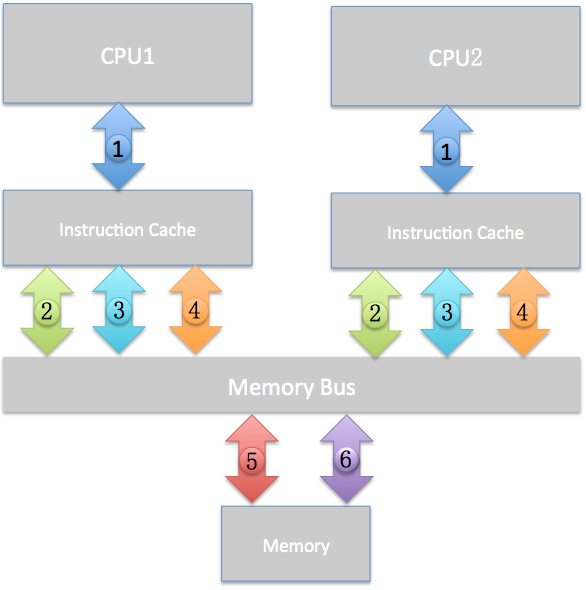
\includegraphics[width=5in]{RTL.png}}
\caption{SoC platform structure.}
\label{rtlstruc}
\end{figure}


 Due to the lack of similar research, we cannot find any existing model with accurate flow specifications,
therefore this model is built from scratch.
Here the flow specifications from GEM5 are slightly modified and applied
to the RTL model shown in Figure~\ref{rtlstruc}.
 This model consists of two CPU models, each with its own 1KB cache.
 The caches are connected to a 4MB memory through a memory bus model.
 Currently, the CPUs are treated as test environment where software programs are simulated to trigger various flows.
 This model is simulated using an open-source simulator for the VHDL language called GHDL.


 To collect communication activities of the system,
 the test environment collects values of selected signals
 into an output trace file on each rising clock edge.
GHDl itself also
outputs a tracing file in format of vcd (value change dump) where
any value changes on all signals are collected, this format
can be opened by wave viewer softwares and provide a 
graphical representation of changes in a recorded signal's amplitude,
Figure~\ref{wave} shows an example of trace in waveform format.
The trace analysis algorithm is modified to be able
to take both format of trace files as input and
perform trace abstraction function on.
 \begin{figure} [h]
\centerline{
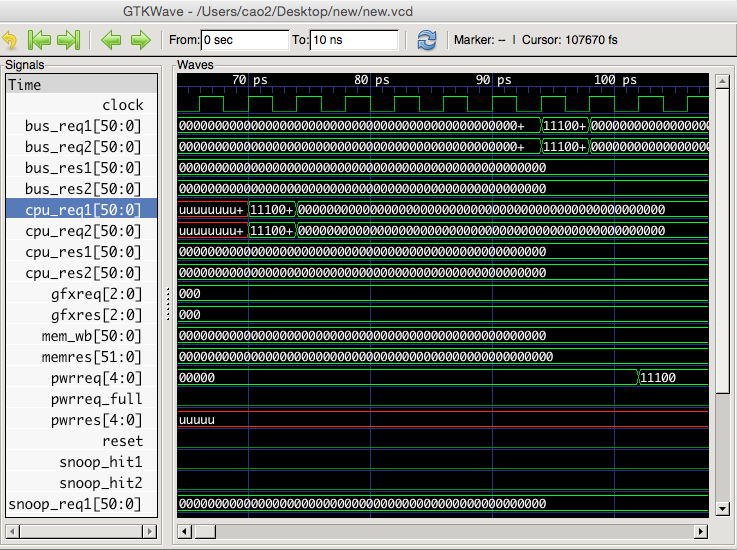
\includegraphics[width=5in]{wave.png}}
\caption{Signal trace in waveform format}
\label{wave}
\end{figure}



There are 6 types of interfaces shown in Figure~\ref{rtlstruc}, each contains multiple signals
that ensures the communications between components.
There are two types of signals, $std\_logic$ that stores only one bit of value and  $std\_logic\_vector$ that
stores a list of bits. This model contains two types of $std\_logic\_vector$, one with width of 51 and another
with width of 52.
  \begin{figure}[h]
\centerline{
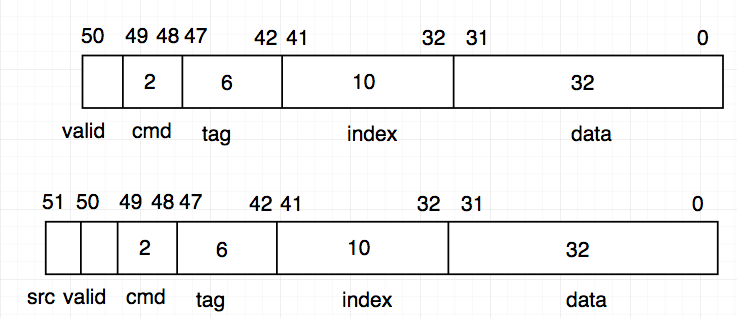
\includegraphics[width=4in]{signalline.png}
}
\caption{Signal bits explaination}
\label{sigline}
\end{figure}
For $std\_logic\_vector$ with 51 bits, as shown in Figure~\ref{sigline},
the most significant bit indicates validity of messages.
The next
two bits 49-48 indicate the command. These two bits can represent four different commands.
Right now our
system supports only two types of commands and
we use 01 to represent read command and 10 to represent write command.
Bits 47-32 represent 16 bits address, and the last 32 bits represent data.
For $std\_logic\_vector$s with 52 bits,
the most significant bit represent source of the request. For example, if a request is from CPU1, that bit
will be 1, otherwise it will be 0, the rest of the bits are the same as the first type of $std\_logic\_vector$.

%\begin{figure}[h]
%\centerline{
%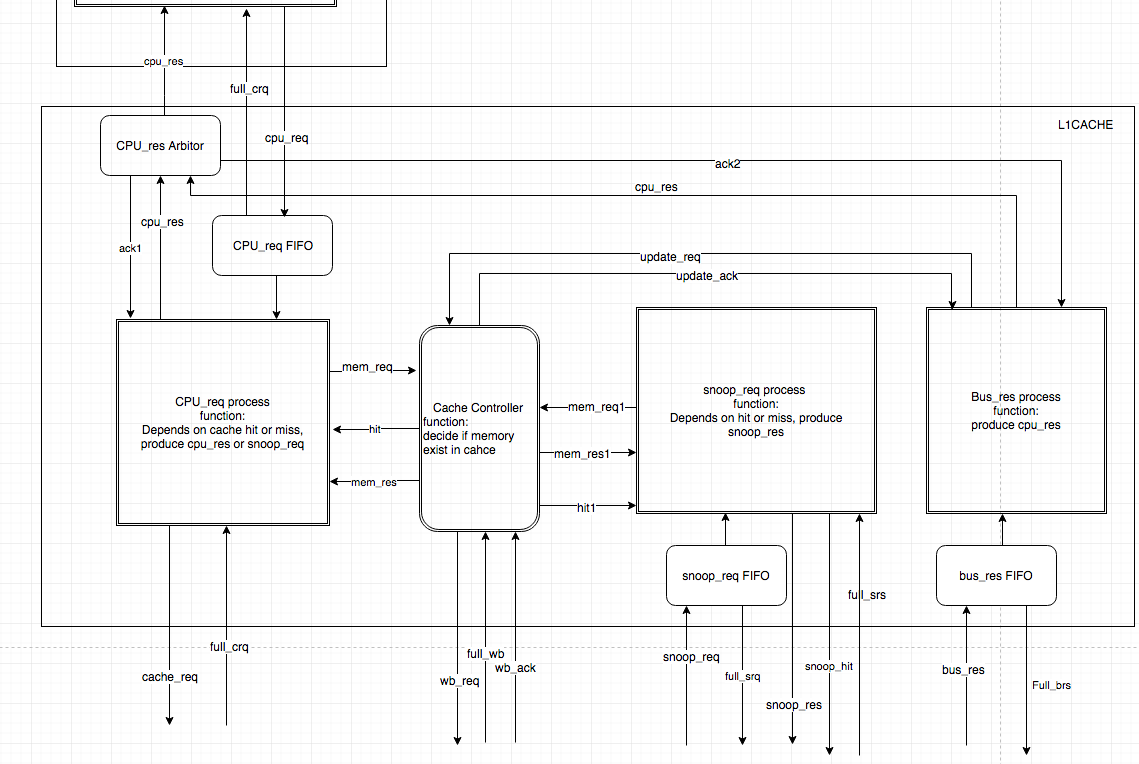
\includegraphics[width=7in]{cache.png}
%}
%\caption{Detailed Cache Structure in RTL Model}
%\label{ccs}
%\end{figure}

The communication between each component are implemented by using handshake protocols to ensure no
data lost. And to implement non-blocking communication, we use
a first in first out (FIFO) buffer inside each component for each incoming signals.
The model shown in Figure~\ref{rtlstruc} has 6 different interfaces, here we explain each interfaces
with signal names and its functionality.
The first interface, as shown in Figure~\ref{int1}, is responsible for communications between CPU and Cache.
There are three signals included in this interface, each of which is explained in Table~\ref{int1t}.
\begin{figure}[h]
\centering
    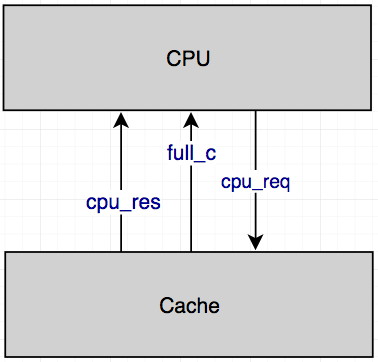
\includegraphics[width=4in]{int1.png}
    \caption{Structure of interface one}
    \label{int1}
 \end{figure}

\begin{table}[h]
\caption{Signals explanations for interface one}

\begin{tabular}{|l|c | p{12cm} |}
\hline
Signal Name & Width & Definition \\
\hline
\hline
$cpu\_req$ 		&$51$			& cpu request from CPU to Cache \\
\hline
$cpu\_res$ 		&$51$			& cpu response from cache to CPU \\
\hline
$full\_c$ 			&$1$				& full indicator of $cpu\_req$ FIFO inside Cache\\
\hline
\end{tabular}
\label{int1t}
\end{table}

There are three interfaces between Cache and Memory Bus. Detailed
structures of these three interfaces are shown in Figure~\ref{int2}.
In this figure, interface two is used for
communications about snoop function, and is composed of those signals with red font;
interface three is used for write back function and is represented in green color;
interface four is in charge of cache requests bus responses, and is
presented in blue color. Signals included in these three interfaces are
explained in Table~\ref{int2t}.
\begin{figure}[h]
\centering
    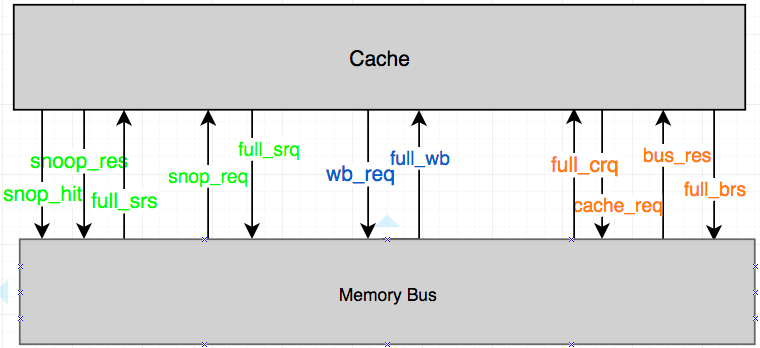
\includegraphics[width=5in]{int2.png}
    \caption{Structure of interface two, three and four}
    \label{int2}
 \end{figure}

\begin{table}[h]
\caption{Signals explanations for interface two, three and four}

\begin{tabular}{|l|l|c | p{12cm} |}
\hline
Interface & Signal Name & Width & Definition \\
\hline
\hline
2 & $snp\_hit$ 			&$1$				& snoop hit signal\\
\hline
2 & $snp\_res$ 			&$51$			& snoop response sent from Cache to Memory Cache \\
\hline
2 & $full\_srs$ 			&$1$				& full indicator of $snp\_res$ FIFO inside Memory Bus\\
\hline

2 &$snp\_req$ 			&$51$			& snoop request sent from Memory Bus to Cache \\
\hline
2 &$full\_srq$ 			&$1$				& full indicator of $snp\_req$ FIFO inside Cache\\
\hline


3 & $wb\_req$ 			&$51$			& write back request from Cache to CPU \\
\hline
3 & $full\_wb$ 			&$1$				& full indicator of $wb\_req$ FIFO inside Memory Bus\\
\hline


4 & $full\_creq$ 			&$1$				& full indicator of $cache\_req$ FIFO inside Memory Bus\\
\hline
4 & $cache\_req$ 			&$51$			& Cache request send to Memory Bus\\
\hline
4 & $bus\_res$ 			&$51$			& bus response from Memory Bus to Cache \\
\hline
4 & $full\_brs$ 			&$1$				& full indicator of $bus\_res$ FIFO inside Cache\\
\hline

\end{tabular}
\label{int2t}
\end{table}
Two interfaces are constructed between memory bus and memory.
Interface five is designed for handling data request functions, and is
composed of signals in color blue in Figure~\ref{int3}.
Interface six is exclusively for write back functions, and is represented in
color red in Figure~\ref{int3}.
Detailed explanations of each signal are explained in
Table~\ref{int3t}.
\begin{figure}[h]
\centering
    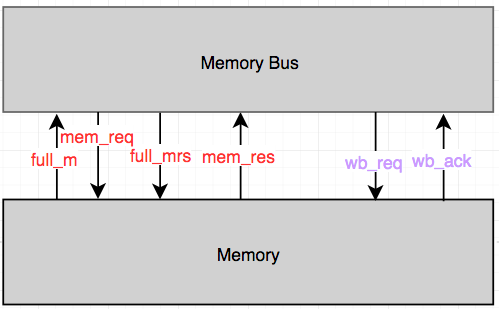
\includegraphics[width=3.5in]{int3.png}
    \caption{Structure of interface five and six}
    \label{int3}
 \end{figure}
\begin{table}[h]
\caption{Signals explanations for interface five and six}

\begin{tabular}{|l|l|c | p{12cm} |}
\hline
Interface & Signal Name & Width & Definition \\
\hline
\hline
5	 &	$full\_m$ 			&$1$				& full indicator of $mem\_req$ FIFO inside Memory\\
\hline
5	 &	$mem\_req$ 			&$52$			& memory request from Memory Bus to Memory, first bit indicate which cache initiate this requirement\\
\hline
5	 &	$full\_mrs$ 			&$1$				& full indicator of $mem\_res$ FIFO inside Memory Bus\\
\hline
5	 &	$mem\_res$ 			&$52$			& memory response from Memory to Memory Bus \\
\hline

6	 &	$wb\_req$ 			&$51$			& Write back request from Memory Bus to Memory\\
\hline
6	 &	$wb\_ack$ 			&$1$				& acknowledgement of write back finished in Memory\\

\hline
\end{tabular}
\label{int3t}
\end{table}

%
% Here we take the L1Cache structure showed in 
%Figure~\ref{ccs} as an example. 
%There are three FIFOs for each input signals: $bus\_res$, $snoop\_req$ and $CPU\_req$ FIFOs.
%Take the $bus\_res \ FIFO$ on the right corner as an example, it has one input $bus\_req$ from memory bus and one
%output $full\_brs$ to memory bus. Before Memory bus want to set $bus\_req$ to valid, it will check the value of $full\_brs$ first.
%If it is set to 1, meaning the FIFO is full, then memory bus will wait until the $full\_brs$ is reset to 0 then set the value of $bus\_req$.
%
%Each of the three FIFOs are connected to its corresponding process that handles
%the incoming signal and produce responses. 
%$Cache\_controller$ process
%manages cache memories. It is in charge of reading and modifying memory data.
%The memory storage in Cache can save up to 1KB memory. The size of the Cache is much smaller than
%actual memory size that can be represented by the 16 bits address, therefore requiring a translation process. As showed in
%Figure~\ref{sigline}, the last 10 bits of address will be used as an index to cache memory vector, while the rest of the 6 will be used
%as an comparator.


This model has 6 protocols implemented. It's based on the protocols provided by GEM5 with some modification. 3 types of protocols: read, write and write back is implemented for both CPU. Write back protocol is new and will be invoked when Cache need to flush back dirty cache lines.

To test the correctness of the cache coherence protocol, we hard coded a test generator inside
of each CPU. 
For every clock cycle, the test generator inside each CPU will randomly generate a read or write operation. In order to better active and cache coherent protocol, only first 3 bits of the 16 bits request address are random generated, while the rest of the bits are predefined. By limiting the address to a certain range, it's more likely that one CPU will request data that exists in the other CPU.

In this experiment model, full observability is assumed.
After the SoC model finishes 2000 flows for each cpu, there
are totally $122704$ messages collected in the trace file.
The trace analysis takes 10 second to finish processing
all these messages and the peak memory used is 18MB.



Table~\ref{table-case-3} shows the number of flow instances contained in that
scenario for the six 
flows describing cache coherent operations initiated from both CPUs.
\begin{table}[h]
\caption{The number of flow instances derived by the trace analysis with the full observability.}
\begin{center}
\begin{tabular}{|l|c|}
\hline
Flows & $\#$Instances \\
\hline
\hline
CPU1 Read			&  $5090$\\
CPU1 Write				&  $4910$\\
CPU1 Write Back				&  $1270$\\

\hline
CPU2 Read			&  $4932$\\
CPU2 Write				&  $5068$\\
CPU2 Write Back				&  $1211$\\
\hline
\end{tabular}
\end{center}
\label{table-case-3}
\end{table}%



This test case works correctly with no inconsistent message occurred. To better 
test our system, we hard coded a simple software that performs Peterson's Algorithm
inside each CPU. Detailed algorithm is displayed in Figure~\ref{petersons}. 
In this algorithm we have four shared variables: $flag0$, $flag1$, $turn$, and $shared$.
\begin{figure}[h]
\RestyleAlgo{boxruled}
\begin{algorithm}[H]
\DontPrintSemicolon
bool flag[2]=$\{false,false\}$\;
int turn\;
int shared\;
\rememberlines
\end{algorithm}

\begin{minipage}{.5\textwidth}
\begin{algorithm}[H]
\resumenumbering
\DontPrintSemicolon
\nonl \ \ \ \ \ CPU0:\;
\hrule
flag[0]=true\;
turn =1 \;
\While{flag[1] $\wedge$ turn ==1 }{
	busy wait\;
}
shared++\;
flag[0]=false\;
\end{algorithm}
\end{minipage}%
{\LinesNumberedHidden
\begin{minipage}{0.5\textwidth}
\begin{algorithm}[H]
\DontPrintSemicolon
\ \ \ \ \ CPU1:\;
\hrule
flag[1]=true\;
turn =0 \;
\While{flag[0] $\wedge$ turn ==0 }{
	busy wait\;
}
shared++\;
flag[1]=false\;
\end{algorithm}

\end{minipage}
}
\label{petersons}
\caption{Peterson's Algorithm on two CPU}
\end{figure}

Each CPU want to enter the critical section will wait until $flag$ or $turn$ has 
the desired value. When entering the critical section, the variable $shared$ will
be incremented by one.
Each CPU will have a loop inside that keeps running this process.
By running this algorithm N times, the final value of $shared$ should
be 2N, as there will be two CPUs increment $shared$ N times. This
value can be used to check the correctness of the algorithm.
\clearpage
\subsection{Debugging Experience}
During the building of the system, our proposed analysis algorithm
is used as a debugging method to locate implementation problems. Following types of errors
are detected by the algorithm and fixed.
\subsubsection{Bug one: duplicated messages}
When the model was first built, each of the CPU was designed to only issue one
read request and one write request. When the trace is produced and analyzed using
the trace analysis algorithm. The analysis was halted and returned a set of partially
executed scenarios and one inconsistent message. This error happens no matter
how many time we simulate the system.
Two different inconsistent messages occurred and is shown below
\[
\begin{array}{|}
(bus, mem, rd, _)\\
(bus, mem, wr, _)\\
\end{array}
\] 


During the trace analysis, our algorithm shows that the trace will always stop when interconnect send
 request to Memory and the message cannot be mapped to any existing scenarios. The error message
 looks exactly the same as the previous message. We traced the bug to interconnect and find out the request
 wasn't reset correctly.

\subsubsection{Error two: command changed after interconnect bus receive snoop request from Cache}

Our trace analysis algorithm find message from cache to memory cannot map to any existing scenarios in 
multiple runs, and all the stacked messages are snoop response. By debugging the cache component,
we discovered the wrong implemented cache coherent protocol and fixed the error.
\subsubsection{Error three: protocol failure}


When running Peterson's Algorithm to ensure mutual exclusion between two processors, our analysis algorithm 
shows no cache coherence protocol was activated. Based on programers experience, there has to be at least one cache 
coherence flow exist because of the shared locks and variable between two CPUs. 
The unmatched number of cache coherence flows shows an big error in our system implementation
of cache coherence protocol. 

This problem can not be found without programmer's view because no error occurred during trace analysis process.
What we found during the analysis is that no matter how long we run the simulation, the number of read flow keep increasing while
others remain the same. This narrows the root cause to the while loop while the program keep checking values of flag to see
if the CPU can enter the critical section. This means that the
shared variable $flag$ and $turn$ are not holding the correct value.

By looking at each flow event, we found out the two CPU requiring the same address data will
result in each CPU thinking they have the exclusive right of that data.
This is because both CPU issue request the same time, they will not 
find the required data anywhere but the Memory, therefore both of the snoop request
will get a cache miss response. 
The problem is solved by adding another register inside the Memory Bus to check
the same request address situation. For example,
when CPU0 requests an address that CPU1
just requested but have not finished yet, CPU0 will wait until CPU1
finished its flow and then precede with a snoop request to CPU1.

 
 After problem in Error three was fixed, we rerun the system and found fair amount of
 cache coherence protocol activated. However, when each CPU run Peterson's Algorithm
 for three times, the final value of $shared$ was 5, comparing to the expected 6.
 
 By analyzing the flow traces, we could not find any error. Because this problem
 resides in the actual value of the data, which is not considered at all in our algorithm,
 it is very hard to root cause the problem. Here we propose to record the order
 the each flow's start and finishing time. By analyzing this we may be able to
 find the real problem. Another reason why recording the order of flows is beneficial
 is that for future research, we can add assertions about order relation into the analyzing
 process. This will allow us to find the error location before it cause an an consequence.
 The order relation assertion can be provided with debugger's insights.
 

\chapter{Conclusion and Future Works}
This thesis presents a method for post-silicon validation by
interpreting observed raw signal traces at the level of
system flow specifications.  The derived flow execution
scenarios provide more structured information on system
operations, which is more understandable to system
validators.  This information can help to locate design
defects more easily, and also provides a measurement of
validation coverage.

Due to partial observability, this approach may derive a
large number of different flow execution scenarios for a
given signal trace.  Insights from system validators can
help to eliminate some false scenarios due to the partial
observability.  An interesting future direction is
formalization of the validators' insights using temporal
logic on flows so that the validators can express their
intents more precisely and concisely.

The trace analysis approach presented in this thesis needs to
be iterated with different observations selected in
different iterations in order to eliminate the false
scenarios and to root cause system failures as quickly as
possible.  The observation selection and stitching signal
traces of different observations together for the above goal
will also be pursued in the future.





\begin{appendix}

\chapter{Flow specifications and protocols provided by GEM5}
\section{Protocol Specifications in Message Sequence Chart}
\begin{figure}[h]
\centering
 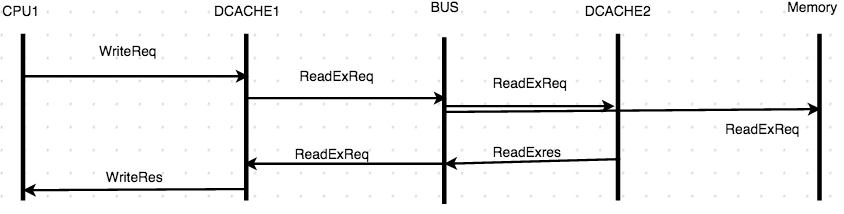
\includegraphics[width=4.5In]{figures/write3.png}
 \caption{\footnotesize Flow sequence chart of write operation when requested data is not included in Dcache. ReadExRes can also be sent from Memory if Dcache2 does not have requested data. This sequence chart is symmetric for CPU2. }
 \label{write3}

 \centering
 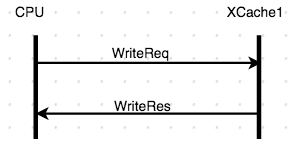
\includegraphics[width=2In]{figures/write1.png}
 \caption{\footnotesize Flow sequence chart of write operation when XCache has the exclusive right of requested data. XCache can be instruction cache or data cache. This sequence chart is symmetric for CPU2. }
 \label{write1}
   \centering
 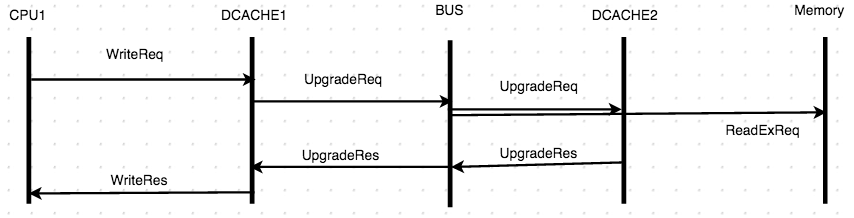
\includegraphics[width=4.6In]{figures/write2.png}
 \caption{\footnotesize Flow sequence chart of write operation when requested data is shared by another component. UpgradeRes can also be sent from Memory if Dcache2 does not have requested data. This sequence chart is symmetric for CPU2. }
 \label{write2}
 \end{figure}
\begin{figure}[h] 
 \centering
 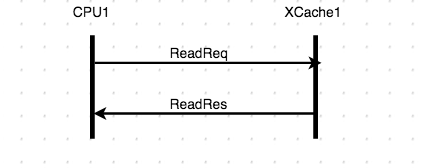
\includegraphics[width=2In]{figures/read1.png}
 \caption{\footnotesize Flow sequence chart of read operation when XCache has the exclusive right of requested data. XCache can be instruction cache or data cache. This sequence chart is symmetric for CPU2. }
 \label{read1}
 
 \centerline{
 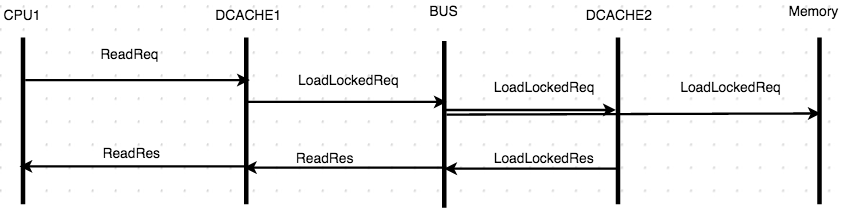
\includegraphics[width=4.1In]{figures/read3.png}}
 \caption{\footnotesize Flow sequence chart of read operation when requested data is shared by another component. LoadLockedRes can also be sent from Memory if Dcache2 does not have requested data. This sequence chart is symmetric for CPU2. }
 \label{read3}

 \centerline{
 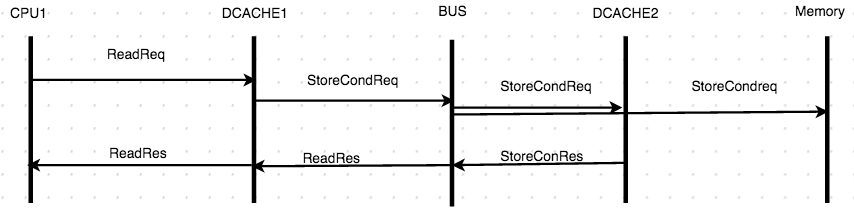
\includegraphics[width=3.9In]{figures/read2.png}}
 \caption{\footnotesize Flow sequence chart of read operation when requested data is not present. StoreCondRes can also be sent from Memory if Dcache2 does not have requested data. This sequence chart is symmetric for CPU2. }
 \label{read2}
 \end{figure}
\newpage
\section{Protocol Specification in LPNs}%
\begin{figure}[h]
\centerline{
 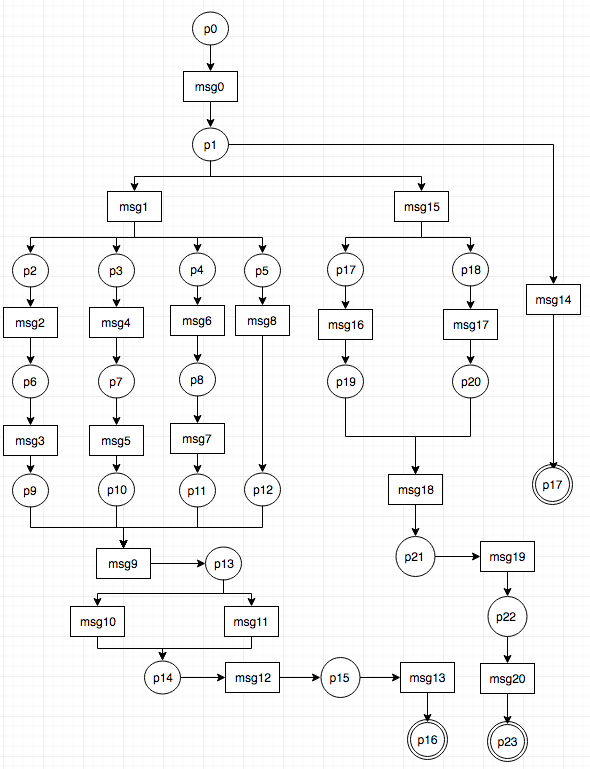
\includegraphics[width=3.1In]{figures/Fig5.png}}%
\begin{minipage}{.5\textwidth}
 {\footnotesize
 \[
 \begin{array}{llll}
 msg_0: (&\mbox{ CPU1},&\mbox{writeReq},&\mbox{icache1   })\\       
 msg_1: (&\mbox{ dcache1},&\mbox{ readExreq },&\mbox{Bus     })\\        
 msg_2: (&\mbox{ Bus},&\mbox{ readExreq},&\mbox{ dcahce2 })\\  
 msg_3: (&\mbox{ dcache2},&\mbox{readExreq},&\mbox{cpu2         })\\   
 msg_4: (&\mbox{ Bus},&\mbox{ readExreq},&\mbox{ icahce2           })\\  
 msg_5: (&\mbox{ icache2},&\mbox{readExreq},&\mbox{cpu2 })\\  
 msg_6: (&\mbox{ Bus},&\mbox{ readExreq},&\mbox{ icahce1       })\\     
 msg_7: (&\mbox{ dcache1},&\mbox{readExreq},&\mbox{cpu1           })\\  
 msg_8: (&\mbox{ Bus},&\mbox{ readExreq},&\mbox{ Memory })\\  
 msg_9: (&\mbox{ true                                          })\\  
 msg_{10}: (&\mbox{ Memory},&\mbox{ readExres},&\mbox{ Bus})
  \end{array}
 \]}
\end{minipage}
\begin{minipage}{.5\textwidth}
 {\footnotesize
 \[
 \begin{array}{llll}
 msg_{11}: (&\mbox{ icache2},&\mbox{ readExres},&\mbox{ Bus })\\  
 msg_{12}: (&\mbox{ Bus},&\mbox{ readExres},&\mbox{ dcache1})\\  
 msg_{13}: (&\mbox{ icache1},&\mbox{ writeRes},&\mbox{ CPU1         })\\  
 msg_{14}: (&\mbox{ icache1},&\mbox{ writeRes},&\mbox{ CPU1 })\\  
 msg_{15}: (&\mbox{ dcache1},&\mbox{UpgradeReq},&\mbox{Bus})\\  
 msg_{16}: (&\mbox{ Bus},&\mbox{ UpgradeReq},&\mbox{ icahce2      })\\   
 msg_{17}: (&\mbox{ Bus},&\mbox{ UpgradeReq},&\mbox{ Memory })\\  
 msg_{18}: (&\mbox{ icache2},&\mbox{UpgradeRes},&\mbox{ Bus     })\\  
 msg_{19}: (&\mbox{ Bus},&\mbox{ UpgradeRes},&\mbox{ dcache1      })\\  
 msg_{20}: (&\mbox{ icache1},&\mbox{ writeRes},&\mbox{ CPU1 })\\
 \\
 \end{array}
 \]}
\end{minipage}
 \caption{\footnotesize Flow specification of a cache coherent write operation initiated from CPU1 to instruction cache. \footnotesize This flow is symmetric for CPU2. }
 \label{write-flow}
 \end{figure}
 \begin{figure}
 \centering
  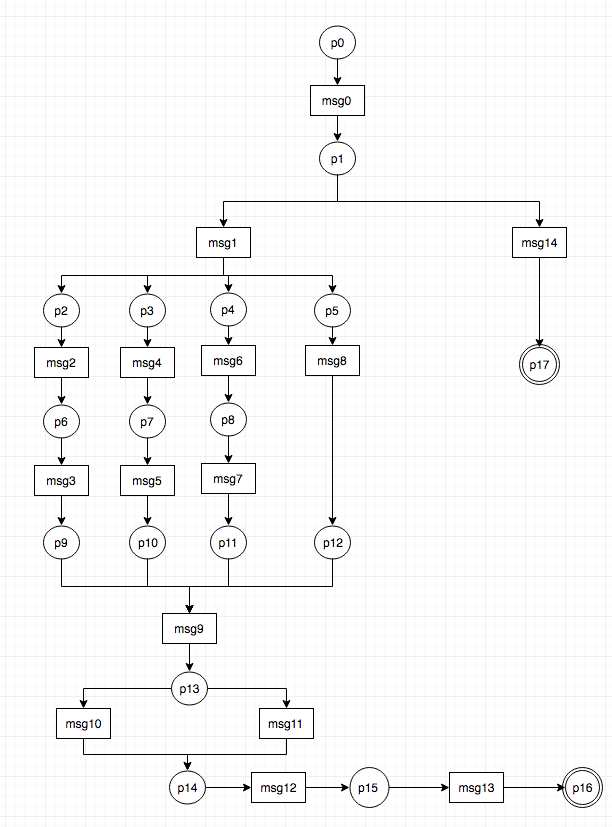
\includegraphics[width=3.3in]{figures/Fih6.png}
  \begin{minipage}{.5\textwidth}
 {\footnotesize
 \[
 \begin{array}{llll}
 msg0: (&\mbox{ CPU1},&\mbox{ReadReq},&\mbox{icache1  })\\                   
 msg1: (&\mbox{ dcache1},&\mbox{ StoreCondreq },&\mbox{Bus })\\           
 msg2: (&\mbox{ Bus},&\mbox{ StoreCondreq},&\mbox{ icahce2 })\\
 msg3: (&\mbox{ icache2},&\mbox{StoreCondreq},&\mbox{cpu2       })\\      
 msg4: (&\mbox{ Bus},&\mbox{ StoreCondreq},&\mbox{ dcahce2           })\\ 
 msg5: (&\mbox{ dcache2},&\mbox{StoreCondreq},&\mbox{cpu2 })\\
 msg6: (&\mbox{ Bus},&\mbox{ StoreCondreq},&\mbox{ dcahce1     })\\       
 msg7: (&\mbox{ icache1},&\mbox{StoreCondreq},&\mbox{cpu1           })
  \end{array}
 \]}
 \end{minipage}%
 \begin{minipage}{.5\textwidth}
  {\footnotesize
 \[
 \begin{array}{llll}
 msg8: (&\mbox{ Bus},&\mbox{ StoreCondreq},&\mbox{ Memory })\\
 msg9: (&\mbox{ true                                        })\\
 msg10: (&\mbox{ Memory},&\mbox{ ReadRes},&\mbox{ Bus            })\\    
 msg11: (&\mbox{ icache2},&\mbox{ ReadRes},&\mbox{ Bus })\\
 msg12: (&\mbox{ Bus},&\mbox{ ReadRes},&\mbox{ dcache1      })\\            
 msg13: (&\mbox{ icache1},&\mbox{ ReadRes},&\mbox{ CPU1          })\\  
 msg14: (&\mbox{ icache1},&\mbox{ ReadRes},&\mbox{ CPU1 })\\\\
 \end{array}
 \]}
 \end{minipage}
 \caption{\footnotesize Flow specification of a cache coherent read operation initiated from CPU1 to instruction cache. \footnotesize This flow is symmetric for CPU2. }
 \label{read-flow} 
 \end{figure}
 
 \begin{figure}[h] 
 \centerline{
 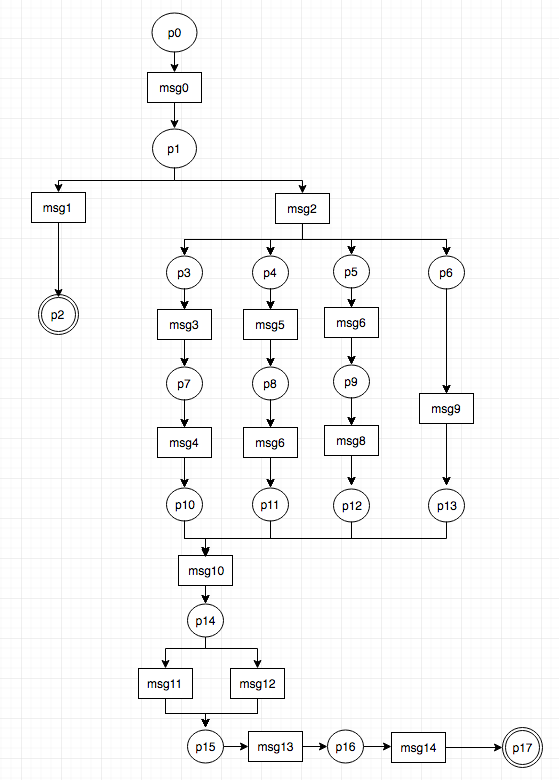
\includegraphics[width=3.3in]{figures/readDcache.png}}
 \begin{minipage}{.5\textwidth}
 {\footnotesize
 \[
 \begin{array}{llll}
 msg0: (&\mbox{ CPU1},&\mbox{ReadReq},&\mbox{dcache1  })\\                   
 msg1: (&\mbox{ dcache1},&\mbox{ ReadRes},&\mbox{ CPU1 })\\
 msg2: (&\mbox{ icache1},&\mbox{ LoadLockedreq },&\mbox{Bus })\\     
 msg3: (&\mbox{ Bus},&\mbox{ LoadLockedreq},&\mbox{ dcahce2     })\\
 msg4: (&\mbox{ dcache2},&\mbox{LoadLockedreq},&\mbox{cpu2 })\\
 msg5: (&\mbox{ Bus},&\mbox{ LoadLockedreq},&\mbox{ icahce2     })\\ 
 msg6: (&\mbox{ icache2},&\mbox{LoadLockedreq},&\mbox{cpu2     })\\
 msg7: (&\mbox{ Bus},&\mbox{ LoadLockedreq},&\mbox{ dcahce1 })

 \end{array}
 \]}
 \end{minipage}\hfill%
  \hfill\begin{minipage}{.5\textwidth}
 
 {\footnotesize
 \[
 \begin{array}{llll}
 msg8: (&\mbox{ icache1},&\mbox{LoadLockedreq},&\mbox{cpu1       })\\
 msg9: (&\mbox{ Bus},&\mbox{ LoadLockedreq},&\mbox{ Memory     })\\
 msg10: (&\mbox{ true })\\
 msg11: (&\mbox{ Memory},&\mbox{ ReadRes},&\mbox{ Bus       })\\     
 msg12: (&\mbox{ icache2},&\mbox{ ReadRes},&\mbox{ Bus    })\\
 msg13: (&\mbox{ Bus},&\mbox{ ReadRes},&\mbox{ icache1 })\\
 msg14: (&\mbox{ dcache1},&\mbox{ ReadRes},&\mbox{ CPU1 })\\\\
 \end{array}
 \]}
 \end{minipage}
 
 \caption{\footnotesize Flow specification of a cache coherent read operation initiated from CPU1 to  data cache. \footnotesize This flow is symmetric for CPU2. }
 \label{read-dcache} 
 \end{figure}
 \clearpage
 




\chapter{Flow Specifications for RTL model}%
\section{Protocol Specification in Message Sequence Charts}
\begin{figure}[h!] 
\centering
 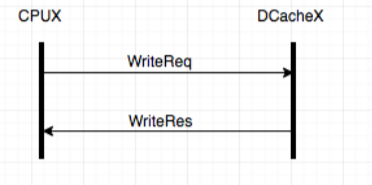
\includegraphics[width=2In]{y1.png}
  \caption{\footnotesize CPU write when cache has exclusive right of the requested data. }
 \label{y1}
 \centering
 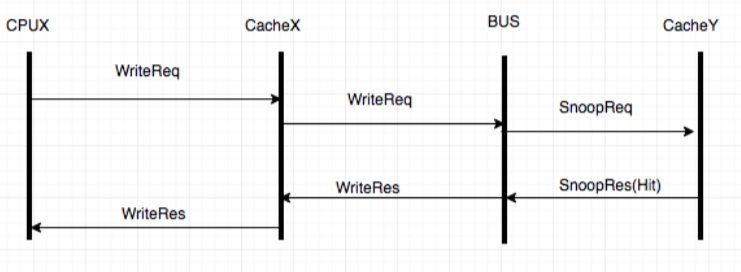
\includegraphics[width=3.6In]{y2.png}
 \caption{\footnotesize CPU write when data only exist in the other CPU's cache }
 \label{y2}
 \centering
 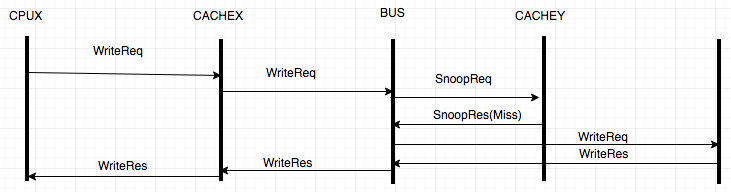
\includegraphics[width=5In]{y3.png}
 \caption{\footnotesize CPU write when requested data only reside in Memory }
 \label{y3}
 \centering
 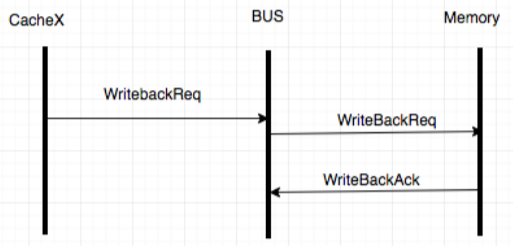
\includegraphics[width=2.8In]{y4.png}
 \caption{\footnotesize Cache send write back request to Memory}
 \label{y4}
\end{figure}

\begin{figure}[h!] 
\centering
 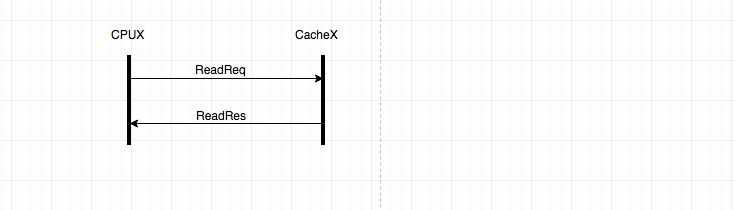
\includegraphics[width=5In]{y5.png}
  \caption{\footnotesize CPU read when cache has exclusive right of the requested data. }
 \label{y4}
 \centering
 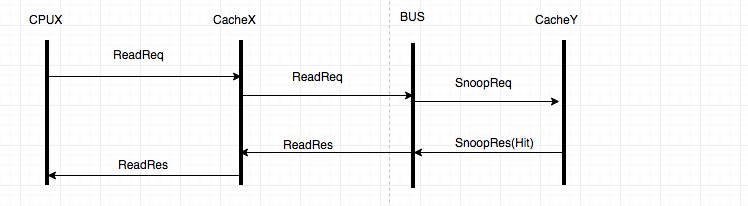
\includegraphics[width=5In]{y6.png}
 \caption{\footnotesize CPU read when data only exist in the other CPU's cache }
 \label{y5}
 \centering
 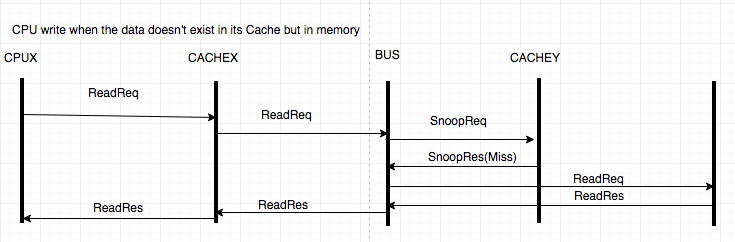
\includegraphics[width=5In]{y7.png}
 \caption{\footnotesize CPU read when requested data only reside in Memory }
 \label{y6}

\end{figure}
 The read and write protocols in RTL model are very similar to what we used in
 GEM5 simulator. However, the command name used here is different.


\section{Protocol Specification in LPNs}

 \begin{figure}[h]
 \centerline{
 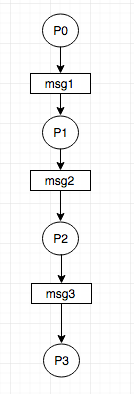
\includegraphics[width=1in]{wbprotocol}}
 {\footnotesize
 \[
 \begin{array}{llll}
 msg1: (&\mbox{ Cache1},&\mbox{ wb },&\mbox{Bus })\\     
 msg2: (&\mbox{ Bus},&\mbox{ wb},&\mbox{ Memory     })\\ 
 msg3: (&\mbox{ Memory},&\mbox{wb},&\mbox{Bus     })\\
 \end{array}
 \]}

  \caption{\footnotesize Flow specification of a cache write back operation initiated from Cache1. \footnotesize This flow is symmetric for CPU2. }
 \label{wbprotocol}
 \end{figure}

\begin{figure}[h]
 \centerline{
 \includegraphics[width=3.2in]{rw}}
 \begin{minipage}{.5\textwidth}
 {\footnotesize
 \[
 \begin{array}{llll}
 msg1: (&\mbox{ CPU1},&\mbox{ wt},&\mbox{ Cache1 })\\
 msg2: (&\mbox{ Cache1},&\mbox{ wt },&\mbox{CPU1 })\\     
 msg3: (&\mbox{ Bus},&\mbox{ snp},&\mbox{ Cache2     })\\
 msg4: (&\mbox{ Cache2},&\mbox{snp},&\mbox{Bus })\\
 msg5: (&\mbox{ Bus},&\mbox{ wt},&\mbox{ Memory     })\\ 
 msg6: (&\mbox{ Memory},&\mbox{wt},&\mbox{Bus     })\\
 \end{array}
 \]}
 \end{minipage}
 \begin{minipage}{.5\textwidth}
 {\footnotesize
 \[
 \begin{array}{llll}
  msg7: (&\mbox{ Bus},&\mbox{ wt},&\mbox{ Cache1 })\\
 msg8: (&\mbox{ Bus},&\mbox{ wt},&\mbox{ Cache1 })\\
 msg9: (&\mbox{ Cache1},&\mbox{wt},&\mbox{CPU1       })\\
 msg10: (&\mbox{ Cache1},&\mbox{wt},&\mbox{CPU1       })\\
 msg11: (&\mbox{ Cache1},&\mbox{wt},&\mbox{CPU1       })\\\\
 \end{array}
 \]}
 \end{minipage}
 \caption{\footnotesize Flow specification of a cache coherent write operation initiated from CPU1 to Cache. \footnotesize This flow is symmetric for CPU2. }
 \label{wtprotocol}
 \end{figure}
\begin{figure}[h]
 \centerline{
 \includegraphics[width=3.2in]{rw}}
\begin{minipage}{.5\textwidth}
 {\footnotesize
 \[
 \begin{array}{llll}
 msg1: (&\mbox{ CPU1},&\mbox{ rd},&\mbox{ Cache1 })\\
 msg2: (&\mbox{ Cache1},&\mbox{ rd },&\mbox{Bus })\\     
 msg3: (&\mbox{ Bus},&\mbox{ snp},&\mbox{ Cache2     })\\
 msg4: (&\mbox{ Cache2},&\mbox{snp},&\mbox{Bus })\\
 msg5: (&\mbox{ Bus},&\mbox{ rd},&\mbox{ Memory     })\\ 
 msg6: (&\mbox{ Memory},&\mbox{rd},&\mbox{Bus     })\\
 \end{array}
 \]}
 \end{minipage}%
 \begin{minipage}{.5\textwidth}
 {\footnotesize
 \[
 \begin{array}{llll}
 msg7: (&\mbox{ Bus},&\mbox{ rd},&\mbox{ Cache1 })\\
 msg8: (&\mbox{ Bus},&\mbox{ rd},&\mbox{ Cache1 })\\
 msg9: (&\mbox{ Cache1},&\mbox{rd},&\mbox{CPU1       })\\
 msg10: (&\mbox{ Cache1},&\mbox{rd},&\mbox{CPU1       })\\
 msg11: (&\mbox{ Cache1},&\mbox{rd},&\mbox{CPU1       })\\\\
 \end{array}
 \]}
 \end{minipage}
 \caption{\footnotesize Flow specification of a cache coherent read operation initiated from CPU1 to Cache. \footnotesize This flow is symmetric for CPU2. }
 \label{readprotocol}
 \end{figure}
 
 
There will be 3 protocols in total: read , write and write back protocl.

All the write operations are implemented in protocol presented in Figure~\ref{wtprotocol}.
When the request activate cache coherent protocol, like in Figure~\ref{y2}, it will end in $state 17$. The rest will end in $state 9$ .


All read operations are implemented in protocol presented in Figure~\ref{readprotocol}. Specification in Figure~\ref{y6} will end in $state 17$. 
The rest of the specification without activating cache coherence protocol end in $state 9$.

\end{appendix}


\begin{spacing}{1}
\bibliographystyle{unsrt}
\bibliography{SoC}
\end{spacing}

\end{document}
